\documentclass[a4paper]{extarticle}
\usepackage[utf8]{inputenc}
\usepackage[a4paper, margin=1in]{geometry}

\usepackage{amssymb}
\usepackage{amsmath}
\usepackage{enumitem}
\usepackage{tcolorbox}
\usepackage{fancyhdr}
\usepackage{graphicx}
\usepackage{float}

\setlength{\parindent}{0em}
\setlength{\parskip}{0.4em}

\definecolor{theoremblue}{RGB}{1, 73, 124}
\definecolor{corollaryblue}{RGB}{70, 143, 175}
\definecolor{exampleblue}{RGB}{137, 194, 217}

\newtcolorbox{tbox}{colback=theoremblue!20,colframe=theoremblue,
boxrule=0pt,arc=0pt,boxsep=2pt,left=2pt,right=2pt,leftrule=2pt}

\newtcolorbox{cbox}{colback=corollaryblue!20,colframe=corollaryblue,
boxrule=0pt,arc=0pt,boxsep=2pt,left=2pt,right=2pt,leftrule=2pt}

\newtcolorbox{ebox}{colback=exampleblue!20,colframe=exampleblue,
boxrule=0pt,arc=0pt,boxsep=2pt,left=2pt,right=2pt,leftrule=2pt}

\title{IntroML - Lecture Notes Week 3}
\author{Ruben Schenk, ruben.schenk@inf.ethz.ch}
\date{\today}

\pagestyle{fancy}
\fancyhf{}
\rhead{ruben.schenk@inf.ethz.ch}
\rfoot{Page \thepage}
\lhead{IntroML - Lecture Notes Week 3}

\begin{document}

\maketitle

\section{Model Selection}

\subsection{Introduction}

\subsubsection{Good Model via Ground Truth}

We formalize again that our goal is to get an intuition for how a sample size \(n\) can change the prediction performance. What is a good prediction? The \textit{goal standard} is to assume the "true" average price is some \textit{ground truth linear function} \(f^*(x) = x^Tw^*\). A \textit{goo model} \(\hat{f}\) is close to the real average \(f^*\), i.e. has a low \textbf{estimation error} \(l(\hat{f}(x), \, f^*(x)) = (\hat{f}(x) - f^*(x))^2\). The average error is then given by \(\mathbb{E}_x(\hat{f}(x)-f^*(x))^2\) over all possible houses \(x\) weighted by how often they might appear. But we don't know \(f^*\), so we can't compute it!

\subsubsection{Prediction Error vs. Estimation Error}

In fact, even though we want to predict the average price \(f^*\) or \(w^*\), we never actually measure it! Instead, we usually only observe \(y_i = f^*(x_i) + \epsilon_i = \langle w^*, \, x_i \rangle + \epsilon_i\) with noise \(\epsilon_i\).

\begin{figure}[H]
    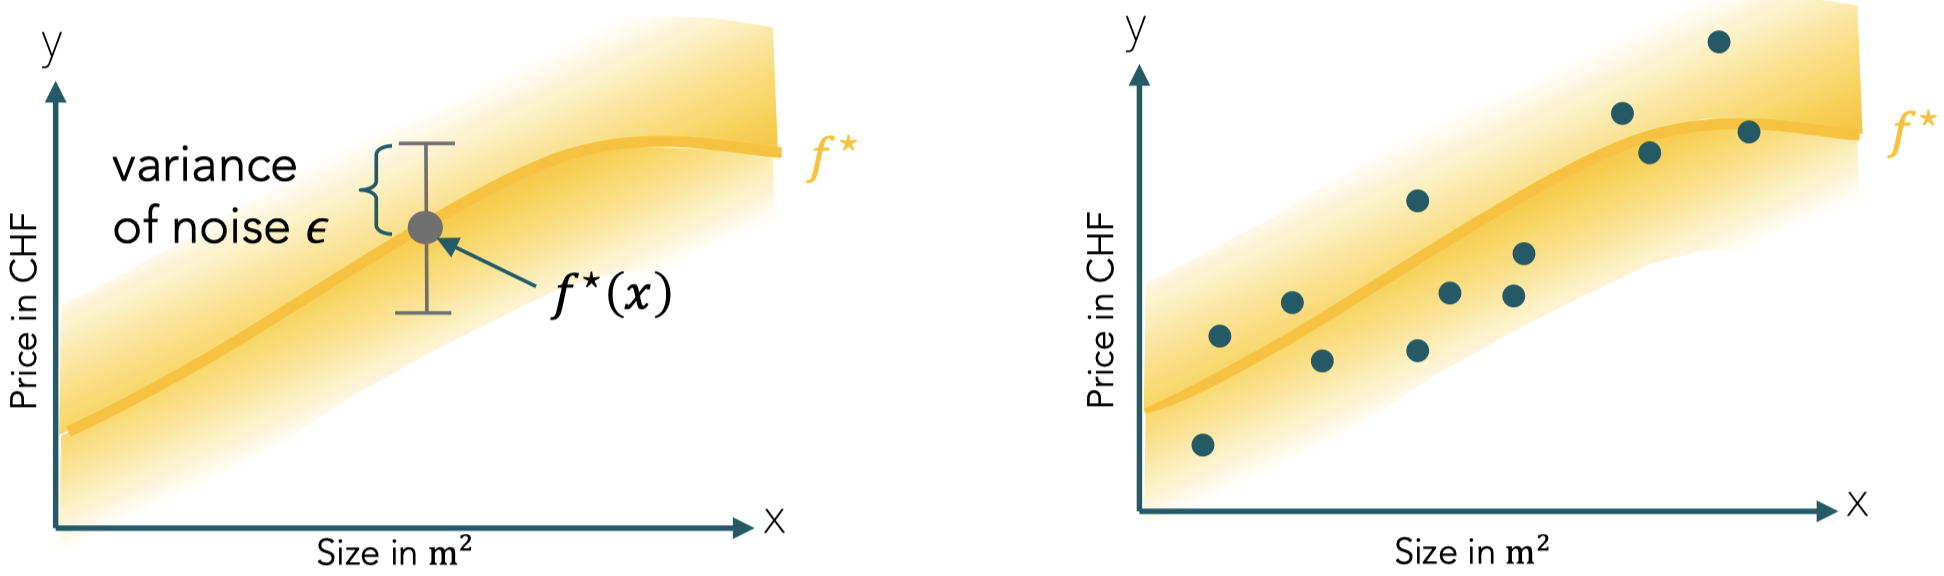
\includegraphics[width=15cm]{../images/IntroML_Fig3-1}
    \centering
\end{figure}

Instead of the estimation error that is predicted compared to the average price \(l(\hat{f}(x), \, f^*(x)) = (\hat{f}(x) - f^*(x))^2\), for each observed sample we can compute the \textbf{prediction error} \(l(\hat{f}(x), \, y) = (\hat{f}(x)-y)^2\). For the following figure, we denote \(e_i = |\hat{f}(x_i)-y_i|\):

\begin{figure}[H]
    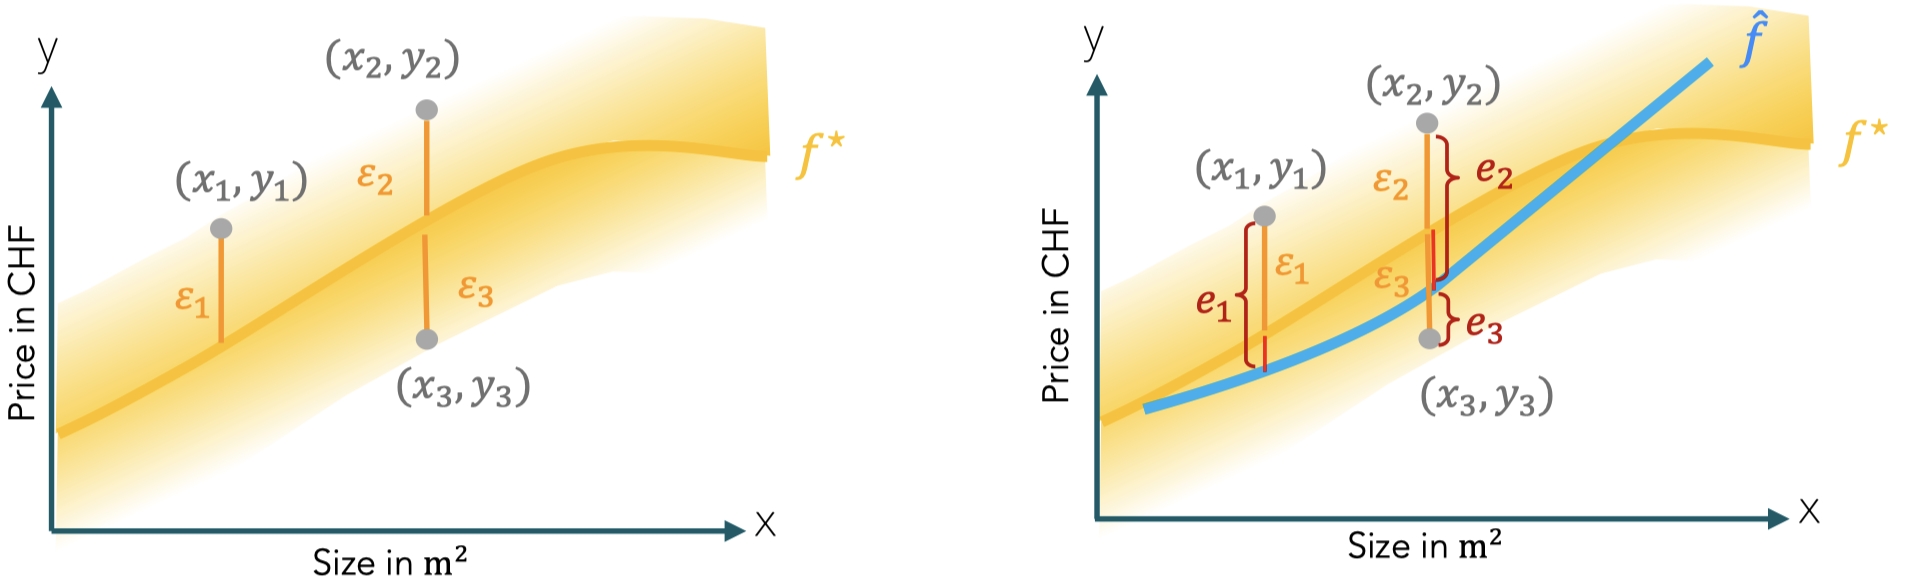
\includegraphics[width=15cm]{../images/IntroML_Fig3-2}
    \centering
\end{figure}

Given the observations \(y = f^*(x) + \epsilon = \langle w^*, \, x \rangle + \epsilon\) we exapnd the square to observations

\[
    l(\hat{f}(x), \, y) = (\hat{f}(x) - f^*(x) - \epsilon)^2 = (\hat{f}(x) - f^*(x))^2 + \epsilon^2 - 2\epsilon(\hat{f}(x) - f^*(x)).
\]

In fact, the \textbf{generalized error} (or average prediction error) is given by

\[
    R(\hat{f}) := \mathbb{E}_{x,y}l(\hat{f}(x), \, y) = \mathbb{E}_xl(\hat{f}(x), \, f^*(x)) + \text{irreducible noise}
\]

\subsection{Objective}

We again remind us about the previously shown pipeline:

\begin{figure}[H]
    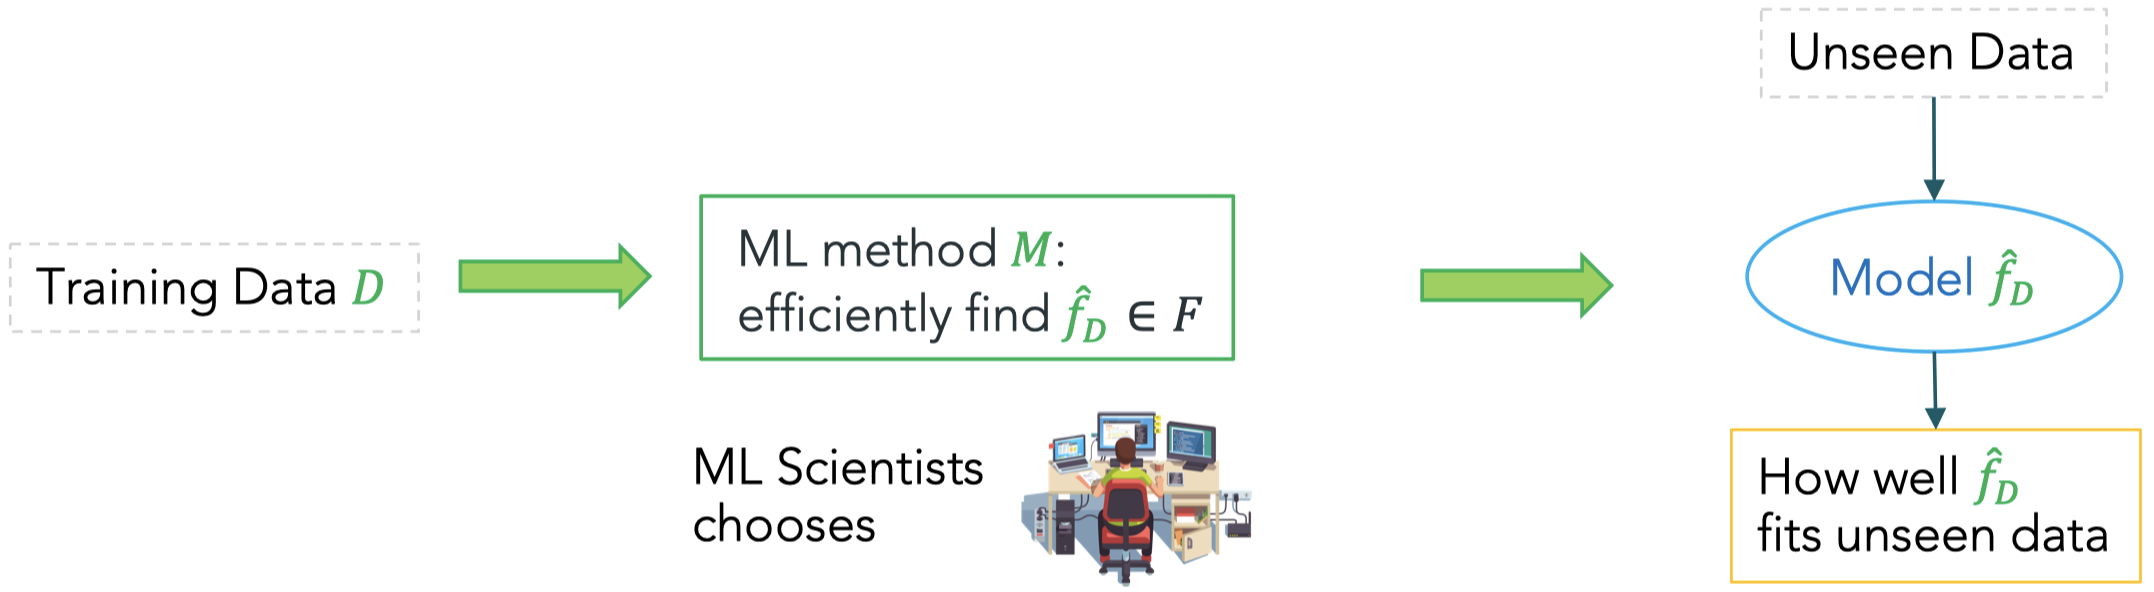
\includegraphics[width=15cm]{../images/IntroML_Fig3-3}
    \centering
\end{figure}

A more precise notation would be: A \textbf{model} \(\hat{f}_D = M(D)\) is obtaine dby using a training method \(M\) on data set \(D\). The  method \(M\) could be, for example, minimizing a particular training loss on \(D\) using a specified optimization algorithm.

\subsection{Approximating Generalization Error}

\subsubsection{Training Loss}

So far, our methods found a minimizer of the training loss \(\hat{f}_D = \arg \min_{f \in F} L(f; \, D) =\\ \frac{1}{n} \sum_{i = 1}^n l(f(x_i), \, y_i)\). However, the training loss \(L(\hat{f}_D, \, D) = \frac{1}{n} \sum_{i = 1}^n l(\hat{f}_D(x_i), \, y_i)\) is in general a \textit{too optimistic} approximation of the generalization error \(R(\hat{f}_D) = \mathbb{E}_{x,y}l(\hat{f}_D(x), \, y)\).

\subsubsection{Simple Train vs. Test Split}

We would like a proxy for the average error on the data that was "unseen" for \(\hat{f}_D\). What we did so far is bad: we were using the training data for both training and evaluation!

The ideas is to \textit{hold out} a part of the available data (called \textbf{held-out or test data} \(D''\)) and only train on the rest \(D = D_{full} - D''\).

Thene, during testing, we approximate the generalization error \(\mathbb{E}_{x, \,y}l(\hat{f}_D(x), \, y)\) by computing the average \textbf{test error} \(\frac{1}{|D''|}\sum_{(x, \, y)\in D''}l(\hat{f}_D(x), \, y)\) evaluated on the test set \(D''\).

\subsubsection{Cross-Validation}

In general we end up with a model selection problem. Consider the scenario for regression where we have no prior knowledge that informs us which feature map \(\phi\) to use. Now we also need to determine which feature map \(\phi\) to use!

The solution is similar to the previous subchapter. We get more stability if we split \(D'\) again in to two sets and then use one to choose the model and one to test the model. I.e., we end up with the following split:

\begin{itemize}
    \item Training set \(D\), usually \(80\%\) or \(50\%\)
    \item Validation set \(D'\), usually \(10\%\) or \(25\%\)
    \item Test set \(D''\), usually \(10\%\) or \(25\%\)
\end{itemize}

Often, the dataset is quite small and it's wasteful to set aside both hold-out validation set and the test set. Instead, with test set \(D''\) fixed, for the rest we choose different validation sets and then average the validation errors.

\paragraph{K-fold cross-validation:} The idea from above is formalized in the \textbf{k-fold cross-validation split}. We first split \(D_{full}\) into \(D_{rest}\) and the test set \(D''\). We then split the rest data into \(K\) same size validation subsets \(D'_k\). We then perform \(k\) splits where the validation set is \(D'_i\) and the training set is \(D_i = D_{rest} \setminus D'_i\) for \(i = 1,..., \, k\).

\begin{figure}[H]
    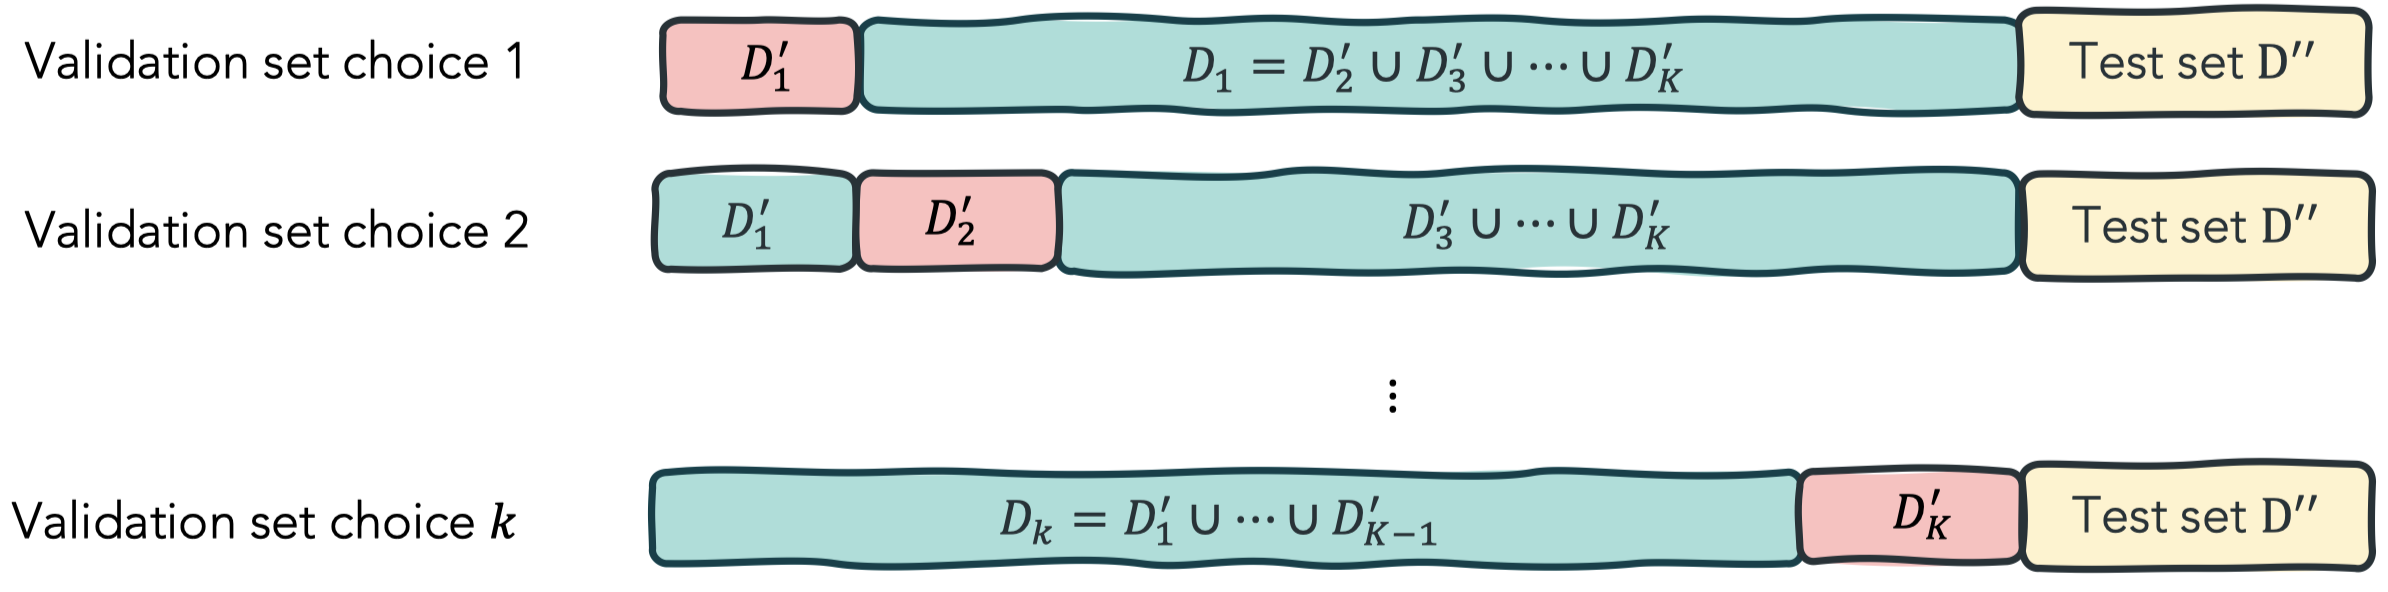
\includegraphics[width=15cm]{../images/IntroML_Fig3-4}
    \centering
\end{figure}

This results in the following algorithm:

\begin{cbox}
    \textbf{Algorithm:} Given a choice of features \(\phi\), and \(K\) folds, do the following steps:
    \begin{enumerate}
        \item For all folds \(k = 1,..., \, K\)
            \begin{enumerate}
                \item Compute \(\hat{f}^{\phi}_k = M_{\phi}(D_k)\) that minimized the training loss on \(D_k\)
                \item Compute the validation error on fold \(k\): \(R_k(\phi) = \frac{1}{|D'_k|} \sum_{(x, \, y) \in D'_k} l(\hat{f}^{\phi}_k (x), \, y)\)
            \end{enumerate}
        \item Compute the \textbf{cross-validation error} \(CV_K(\phi) = \frac{1}{K}\sum_{i = 1}^K R_k(\phi)\)
        \item Model selection: Pick feature \(\phi^*\) with the lowest CV error \(CV_K(\phi)\)
        \item Model training: compute the final model \(\hat{f} = \hat{f}^{\phi^*} = M_{\phi^*(D_{rest})}\)
        \item Model evaluation: estimate generalized error of \(\hat{f}\) using \(D''\) (i.e. \(D_{test}\))
    \end{enumerate}
\end{cbox}

\textit{Note:} This general framework works for comparing any methods \(M\) and losses \(l\). The aim of the model selection is to find a method such that the generalized error \(R(\hat{f})\) is small!

Model selection using CV can work if the CV error of methods \(M_{\phi}\) is close to the generalization error of the method applied to the full dataset. If \(K\) is very large, e.g. \(K = |D_{rest}|\) (\textit{Leave-one-out CV or LOOCV}), we can get the best approxiamtion of \(M_{\phi}(D_{rest})\), since each model \(M_{\phi}(D_k)\) computed in the \(i\)-th split is very similar to \(M_{\phi}(D_{rest})\).
However, this is very computationally intensive, since we need to fit \(|D_{rest}|\) models per method. In practice we typically choose \(K = 5\) or \(K = 10\).

\paragraph{Effects of the choice of k:} The effect of the choice of \(K\) for a fixed method is given in the figure below:

\begin{figure}[H]
    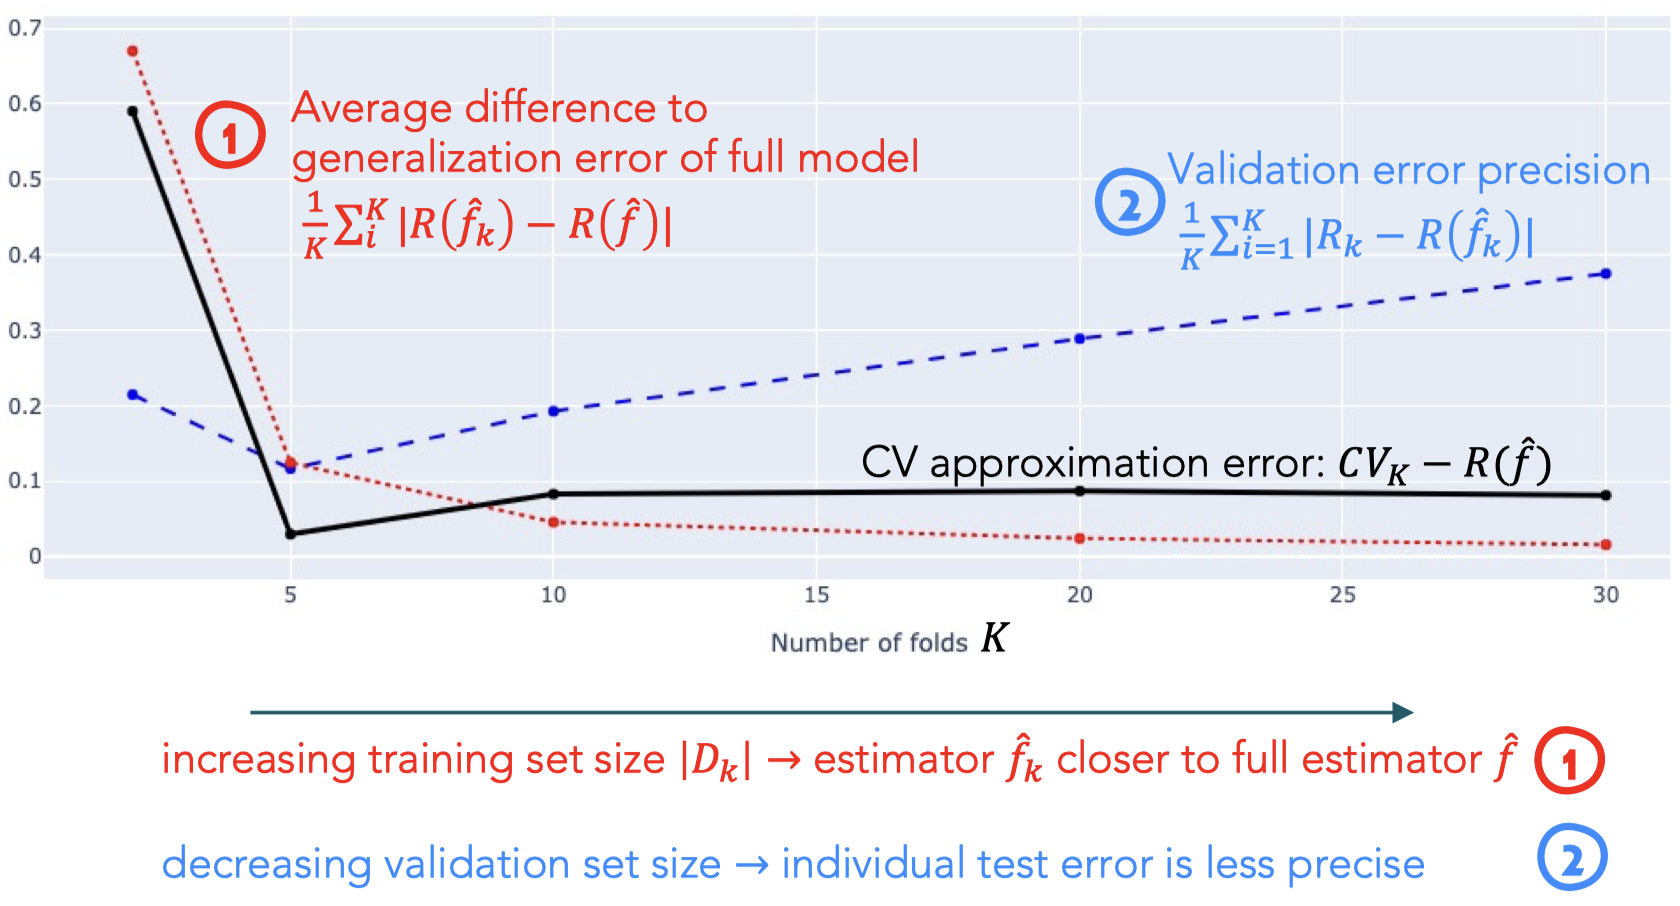
\includegraphics[width=15cm]{../images/IntroML_Fig3-5}
    \centering
\end{figure}

Furthermore, we provide the following notation cheatsheed,for simplicity omitting the dependence on \(\phi\):

\begin{itemize}
    \item Validation error on \(k\)-th split:
    \[R_k = \frac{1}{|D'_k|} \sum_{(x, \, y) \in D'_k}l(\hat{f}_k(x), \, y)\]
    \item Cross-validation error
    \[CV_K = \frac{1}{K} \sum_{i = 1}^K R_k\]
    \item Generalization error for any function \(f\)
    \[R(f) = \mathbb{E}_{x, \, y} l(f(x), \, y)\]
    \item Full estimator
    \[\hat{f} = \arg \min_{f \in F} \sum_{(x, \, y) \in D_{rest}} l(f(x), \, y)\]
\end{itemize}

\subsection{Increasing Model Complexity}

\subsubsection{On The Training Error}

Simplest function (constant):

\begin{figure}[H]
    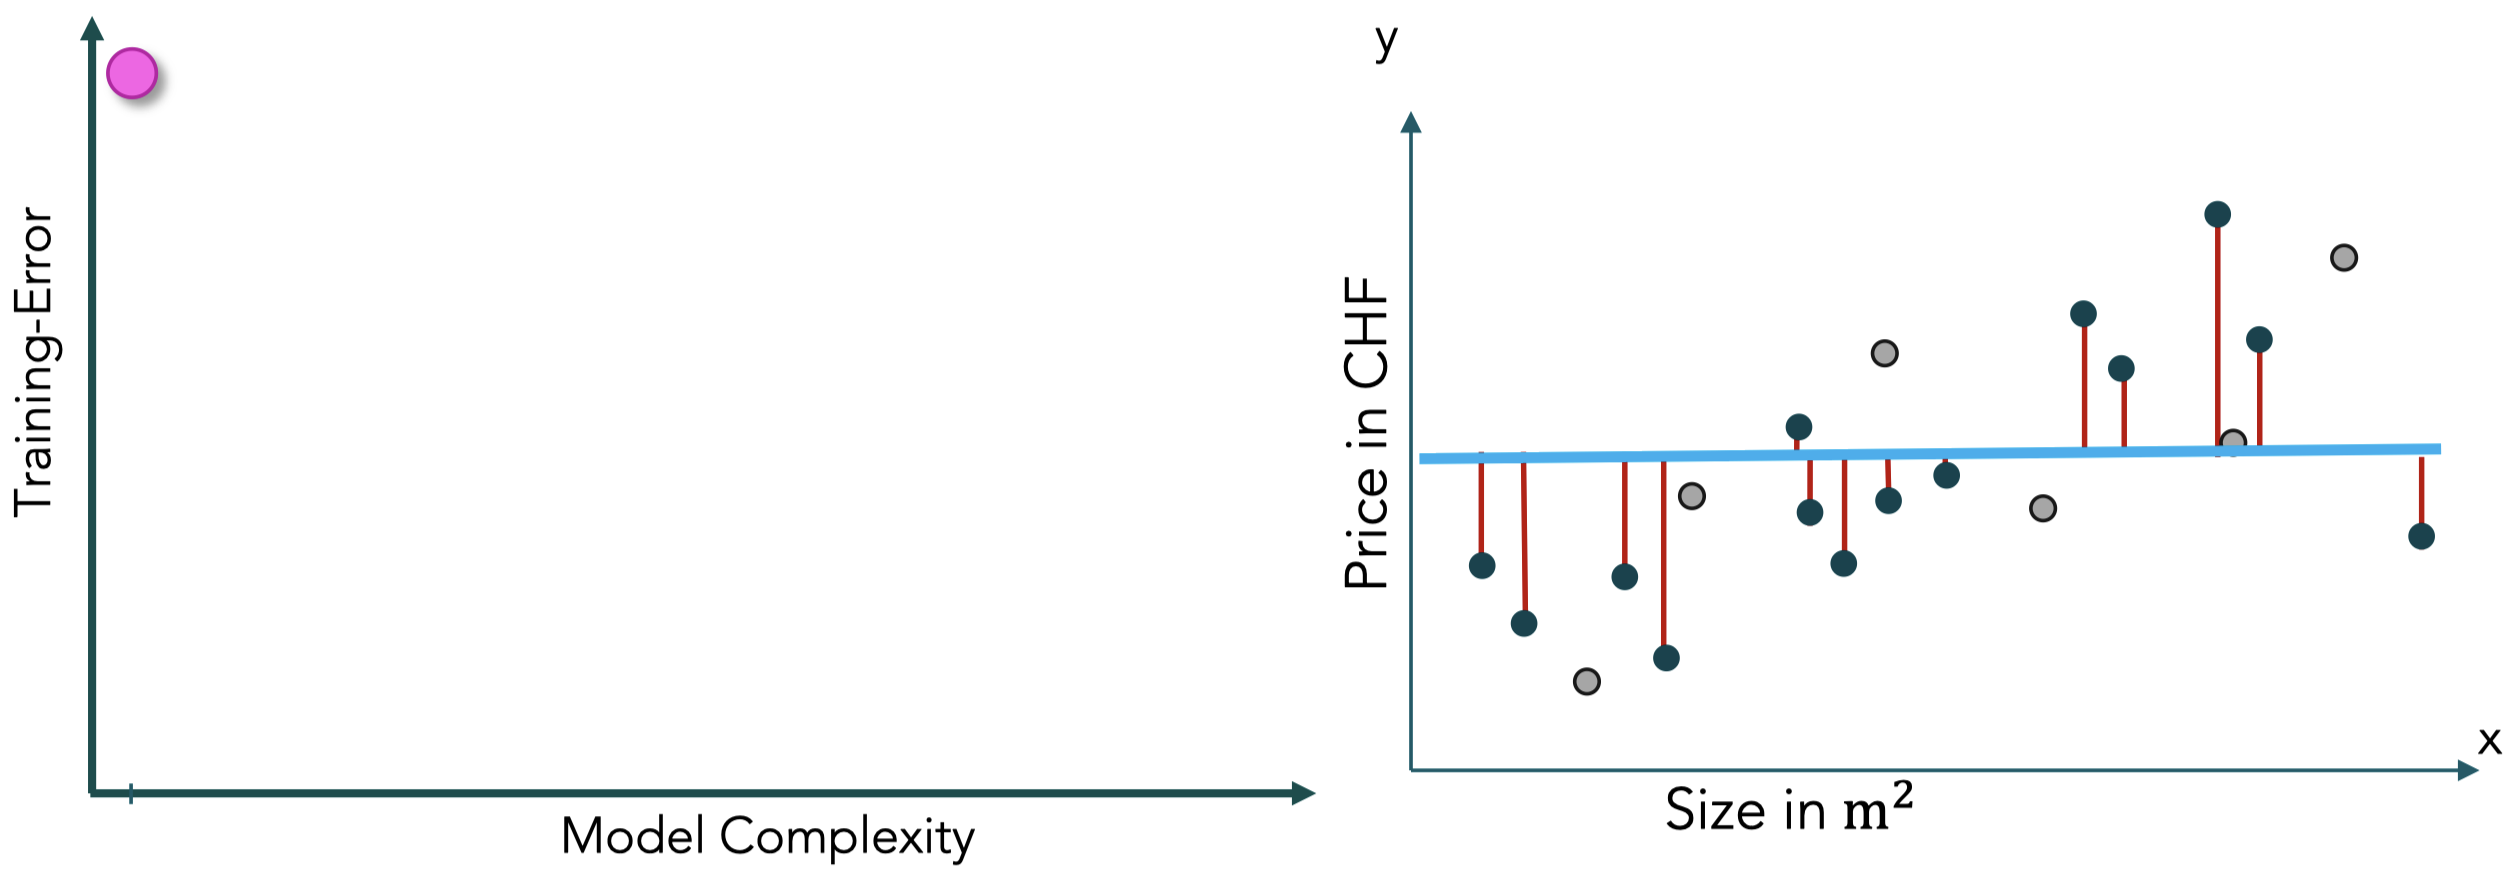
\includegraphics[width=15cm]{../images/IntroML_Fig3-6}
    \centering
\end{figure}

Simple function (linear):

\begin{figure}[H]
    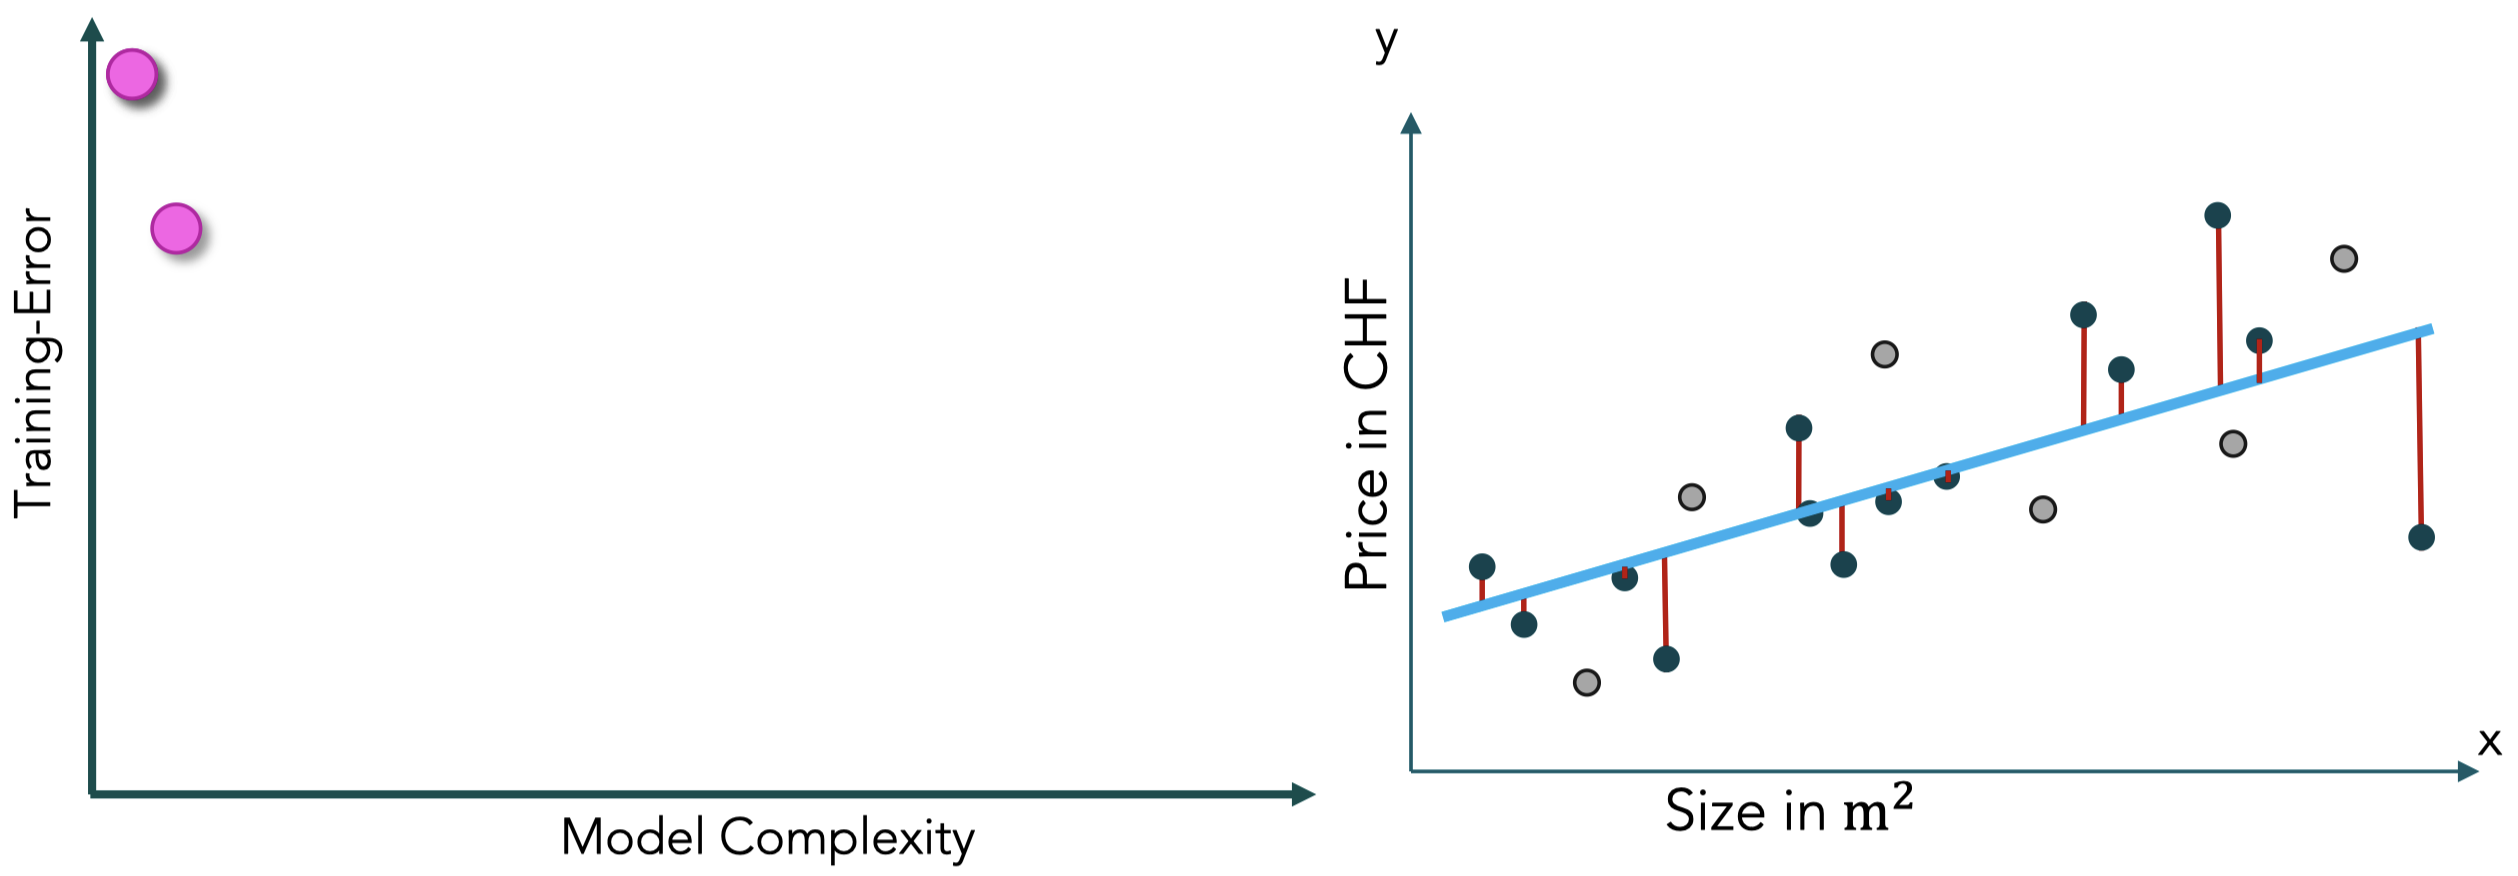
\includegraphics[width=15cm]{../images/IntroML_Fig3-7}
    \centering
\end{figure}

Medium simple function:

\begin{figure}[H]
    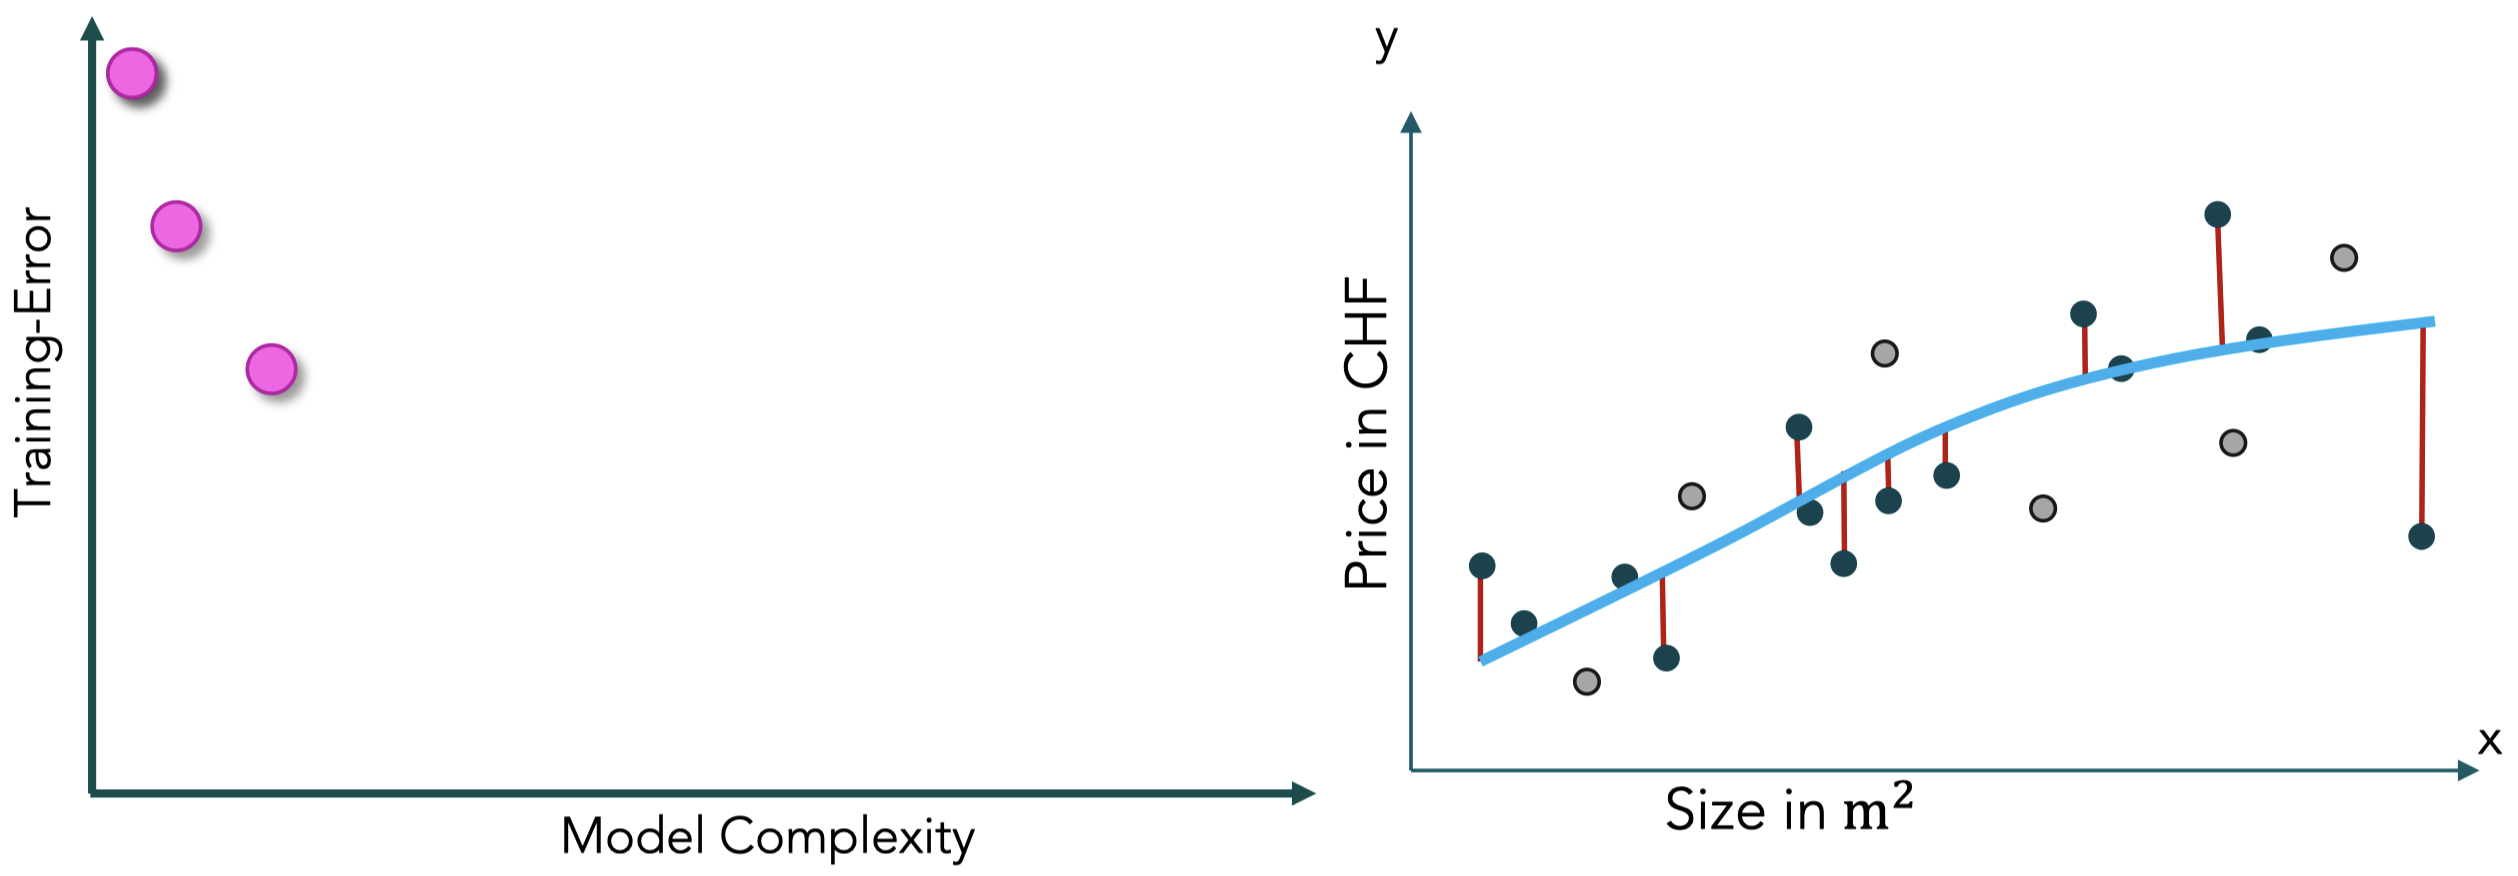
\includegraphics[width=15cm]{../images/IntroML_Fig3-8}
    \centering
\end{figure}

Complex function:

\begin{figure}[H]
    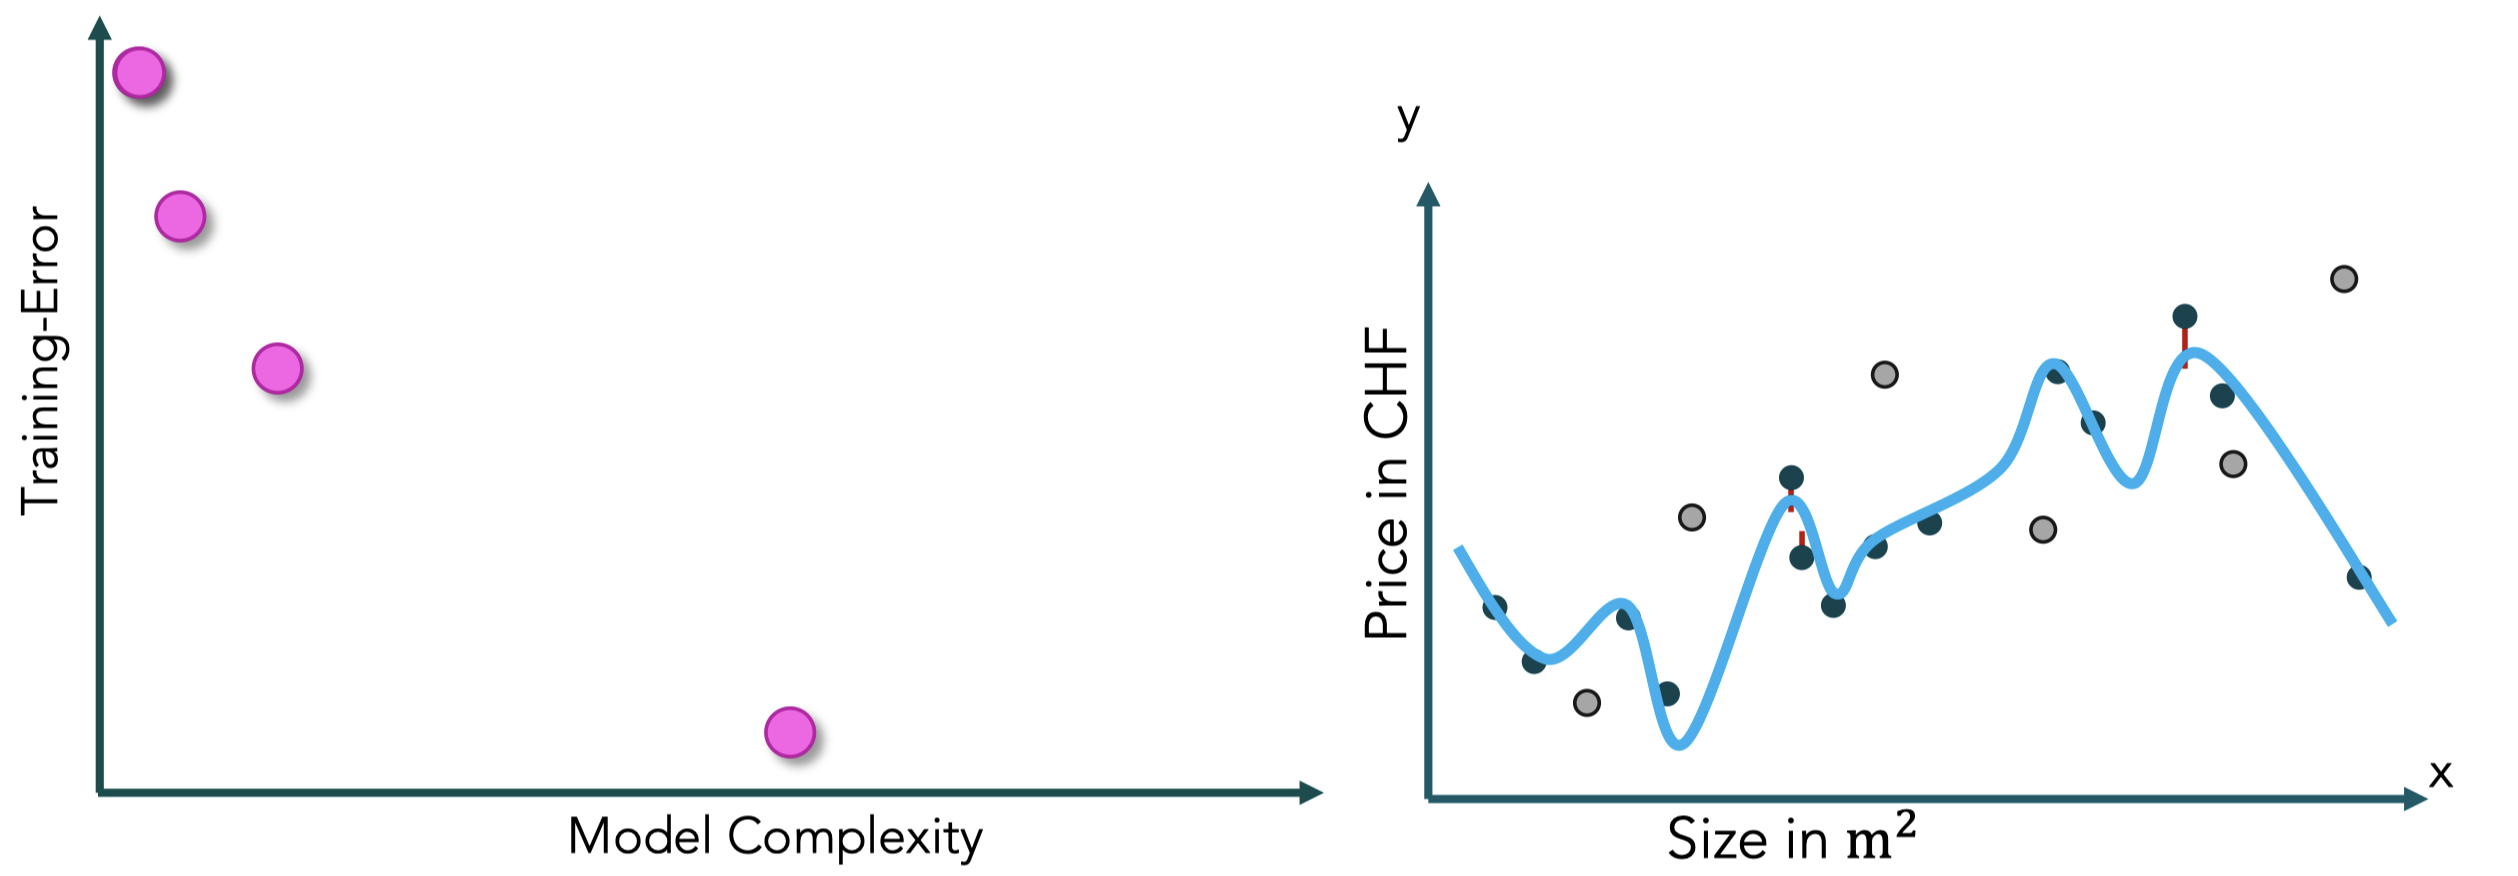
\includegraphics[width=15cm]{../images/IntroML_Fig3-9}
    \centering
\end{figure}

Very complex function:

\begin{figure}[H]
    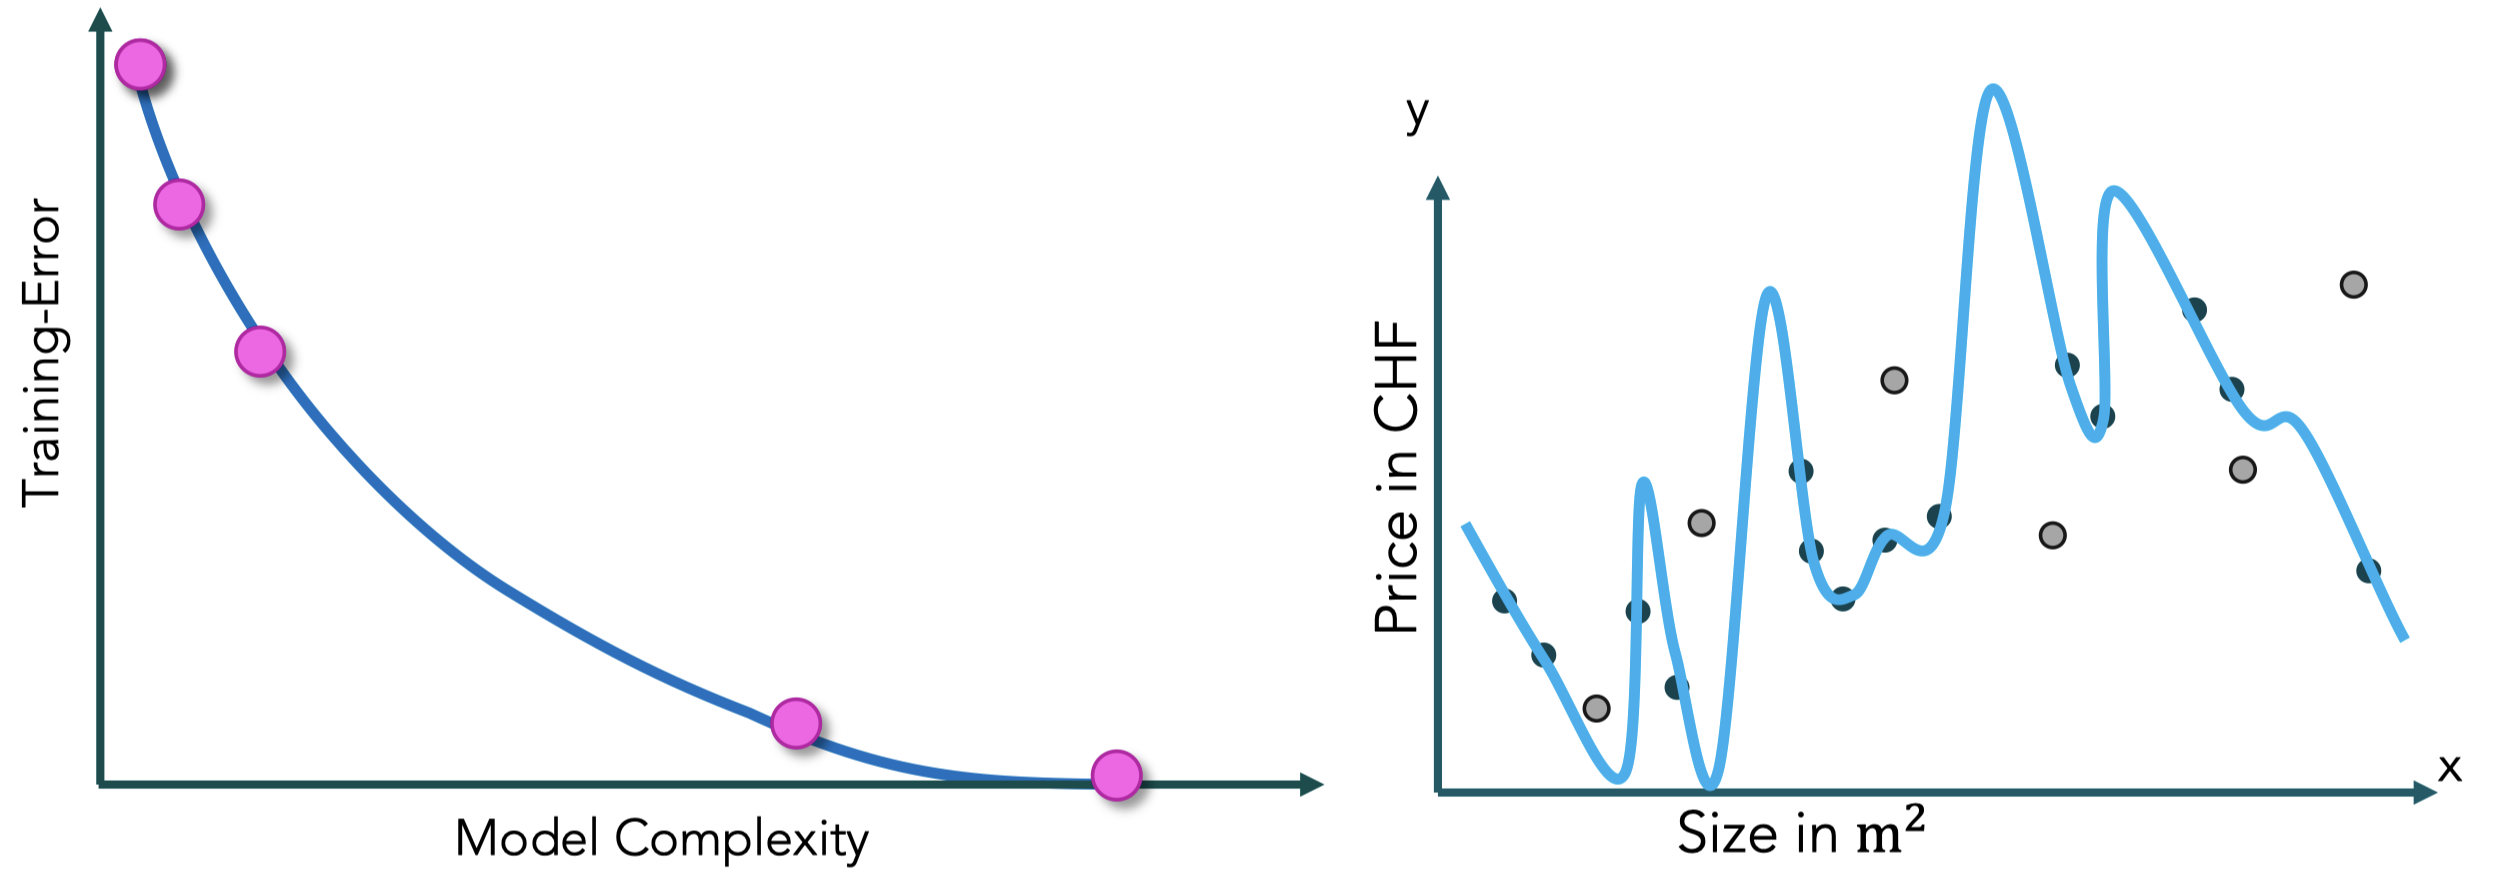
\includegraphics[width=15cm]{../images/IntroML_Fig3-10}
    \centering
\end{figure}

\subsubsection{On The Generalization Error}

Simplest function (constant):

\begin{figure}[H]
    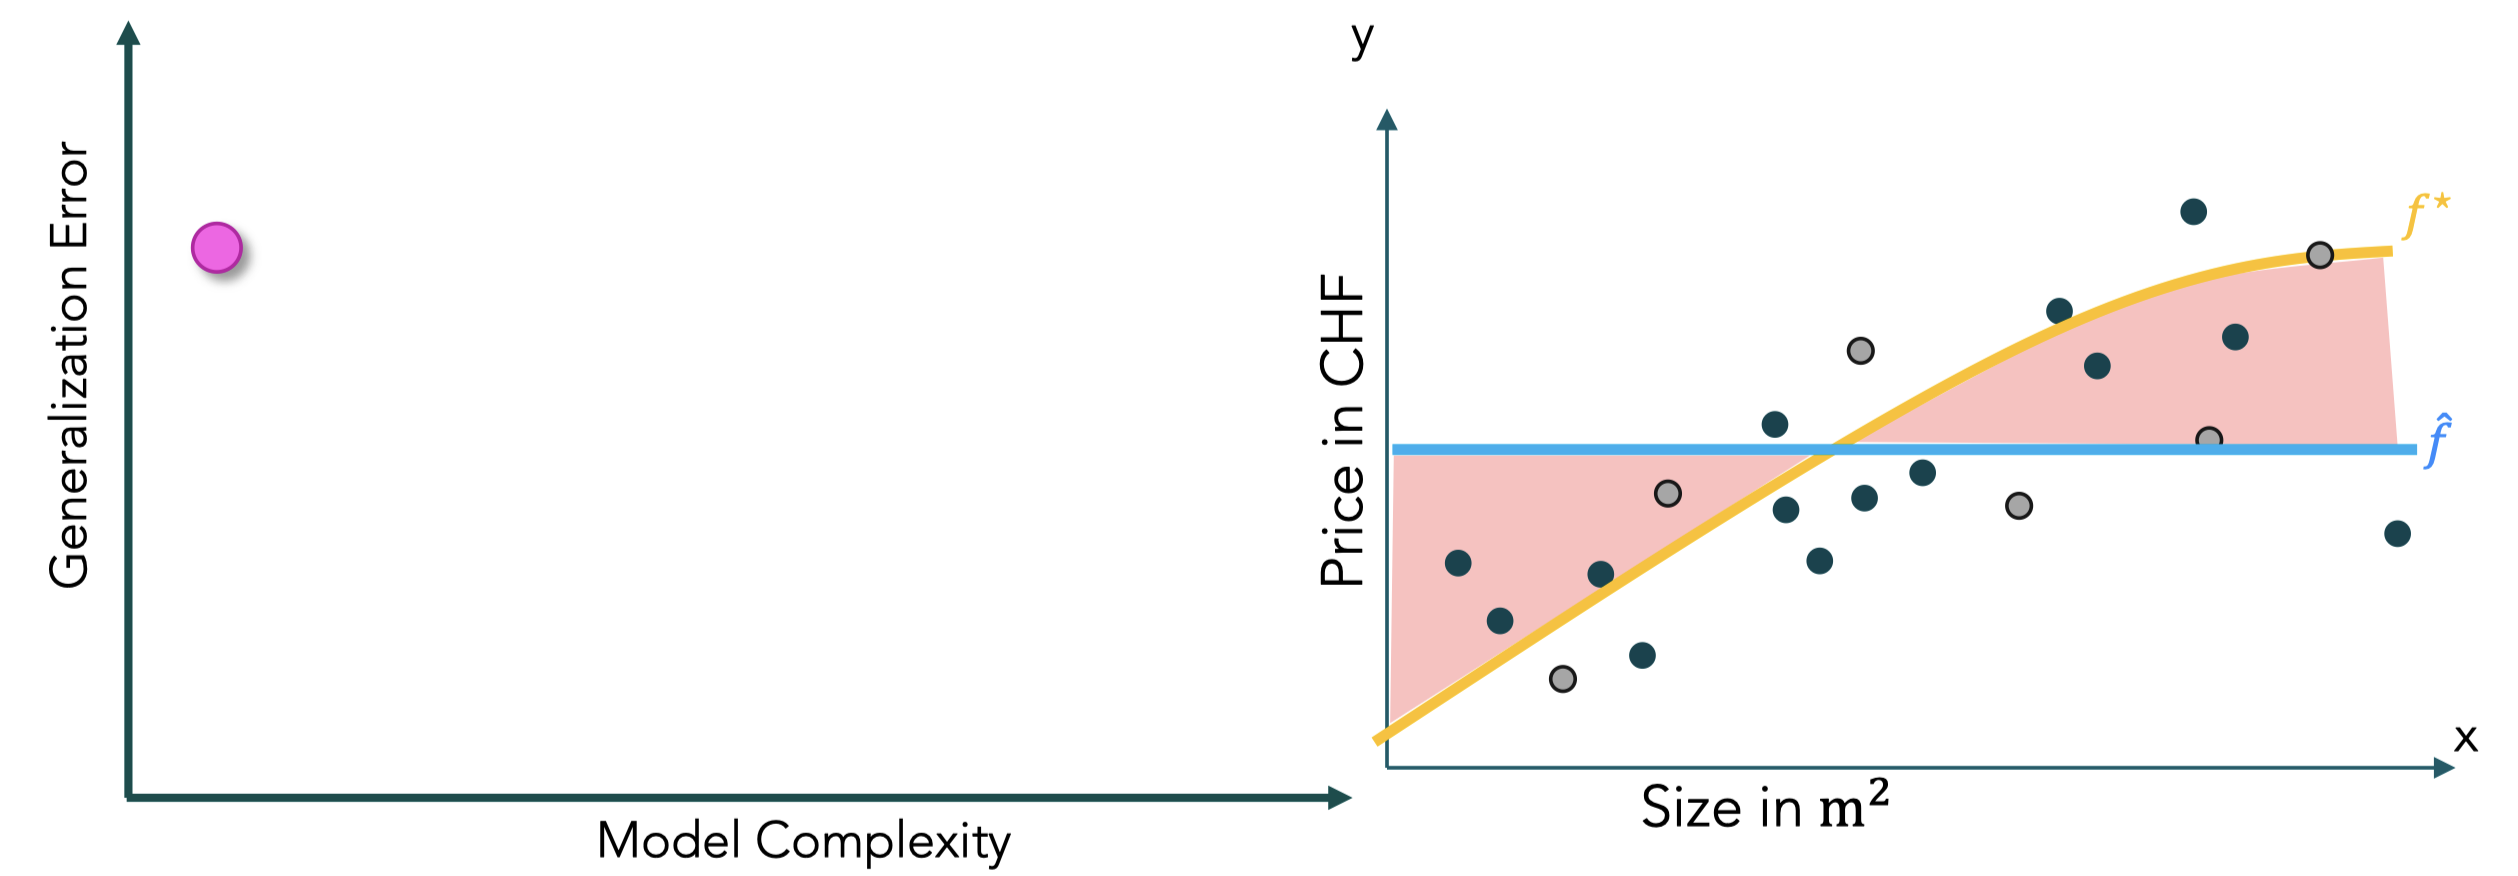
\includegraphics[width=15cm]{../images/IntroML_Fig3-11}
    \centering
\end{figure}

Simple function (linear):

\begin{figure}[H]
    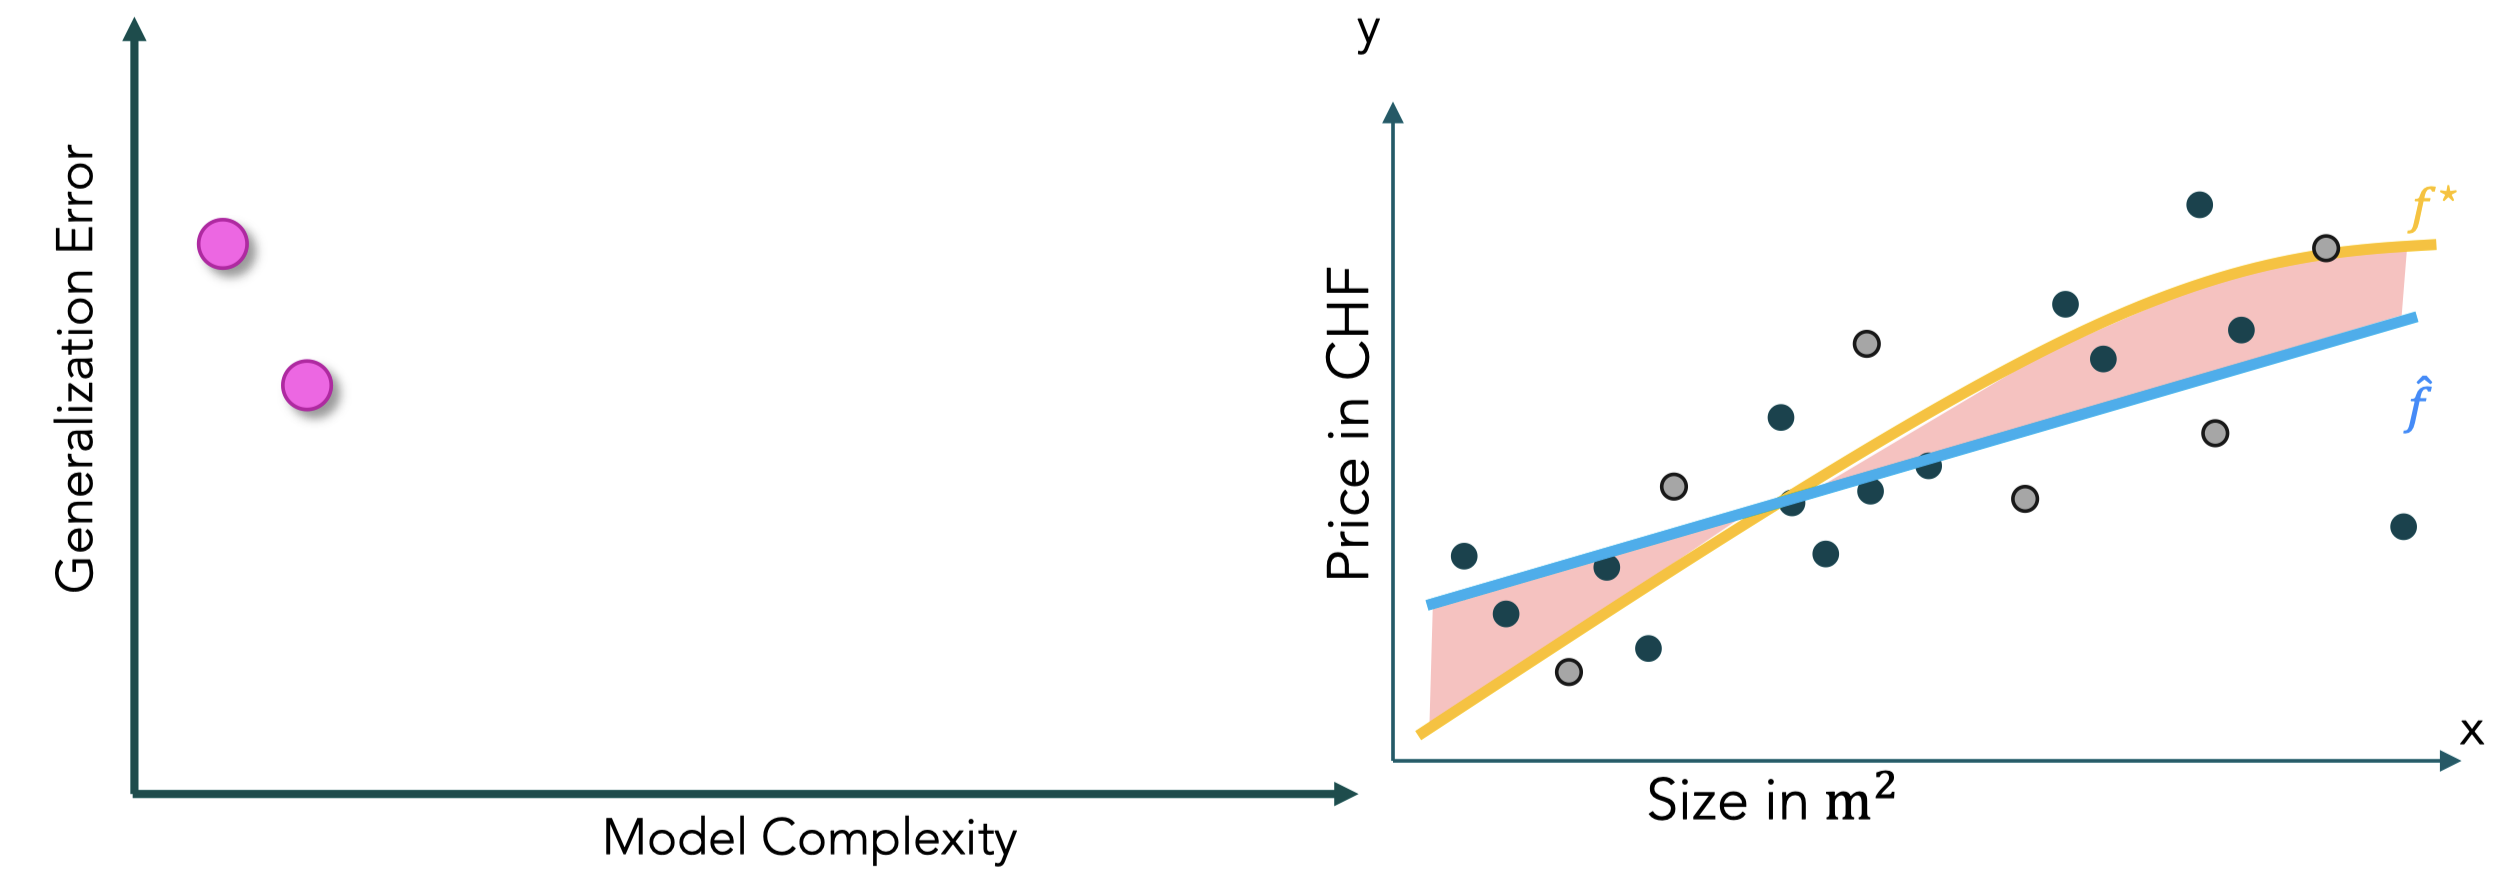
\includegraphics[width=15cm]{../images/IntroML_Fig3-12}
    \centering
\end{figure}

Medium simple function:

\begin{figure}[H]
    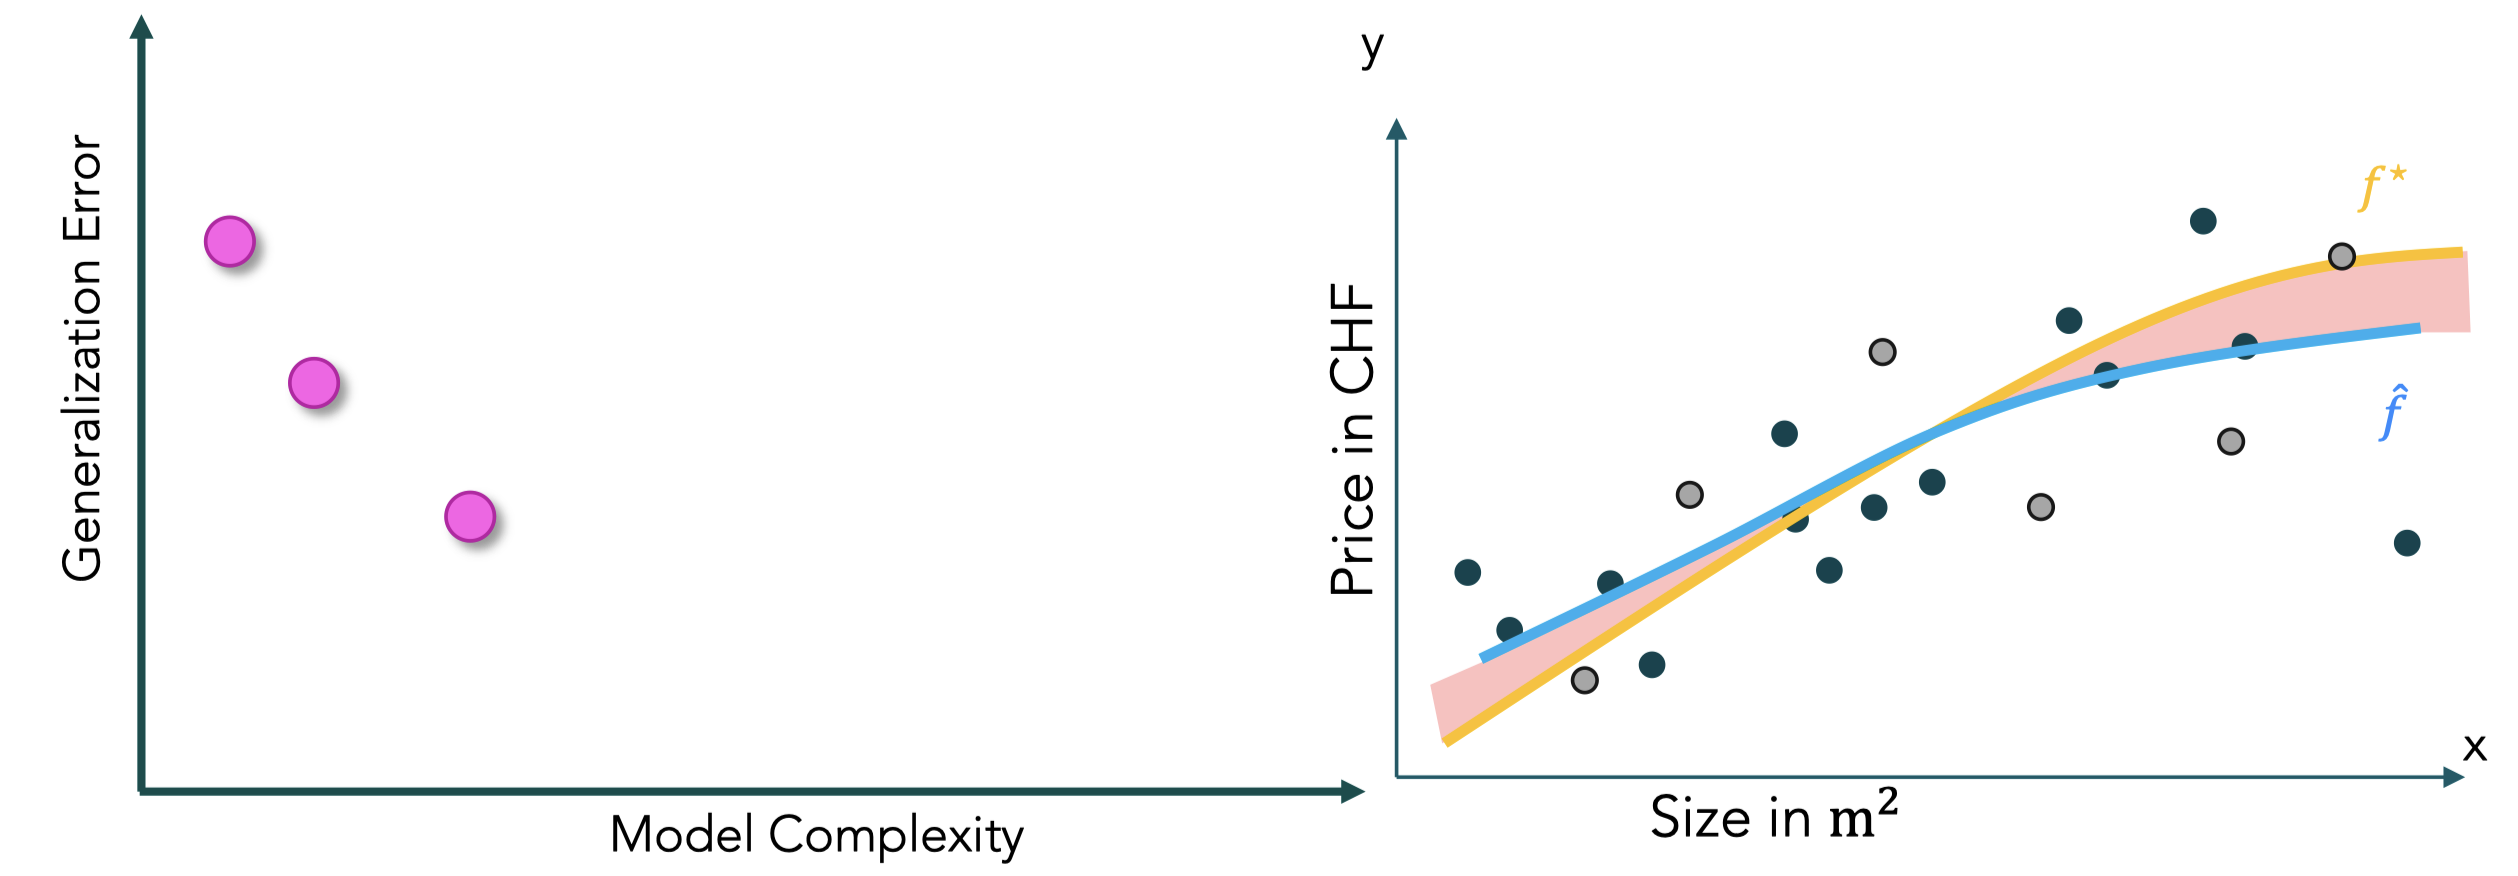
\includegraphics[width=15cm]{../images/IntroML_Fig3-13}
    \centering
\end{figure}

Complex function:

\begin{figure}[H]
    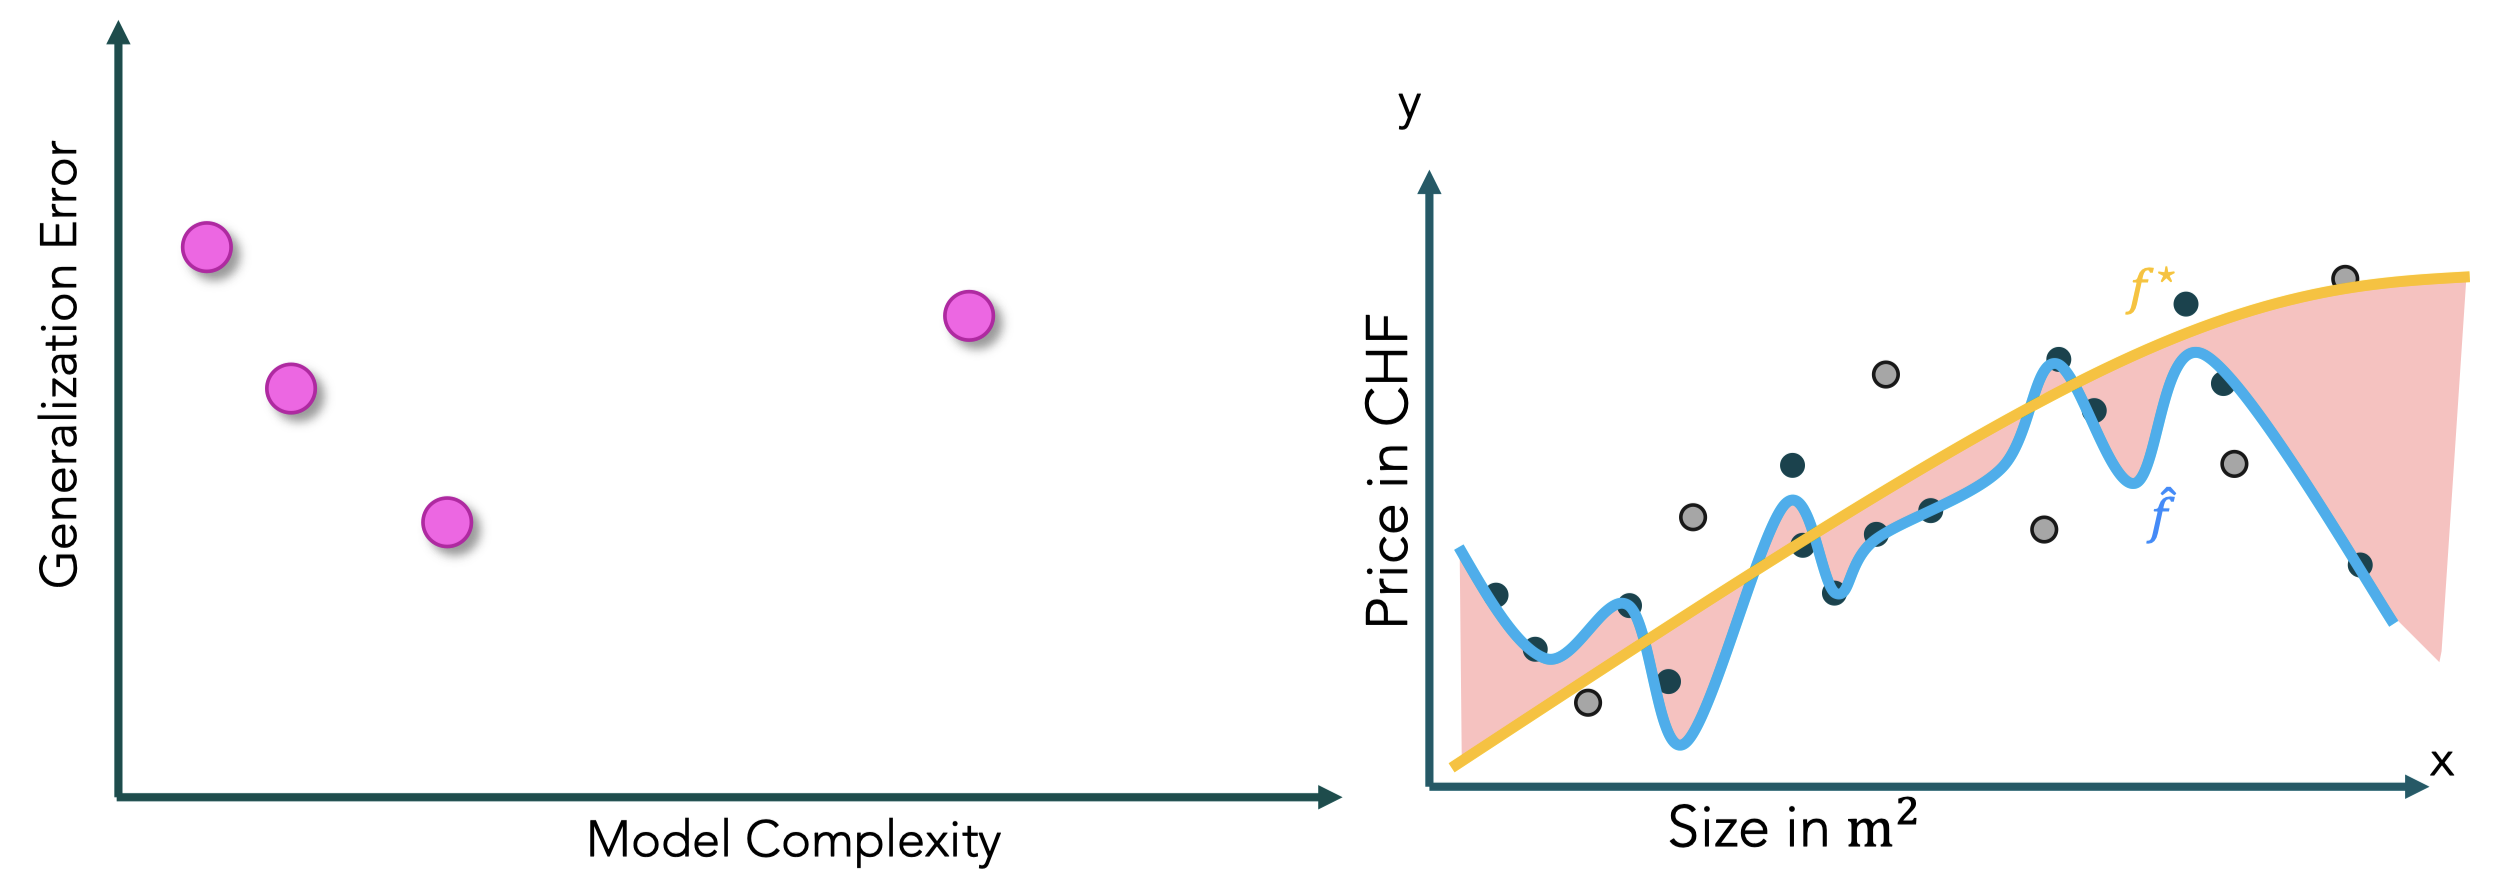
\includegraphics[width=15cm]{../images/IntroML_Fig3-14}
    \centering
\end{figure}

Very complex function:

\begin{figure}[H]
    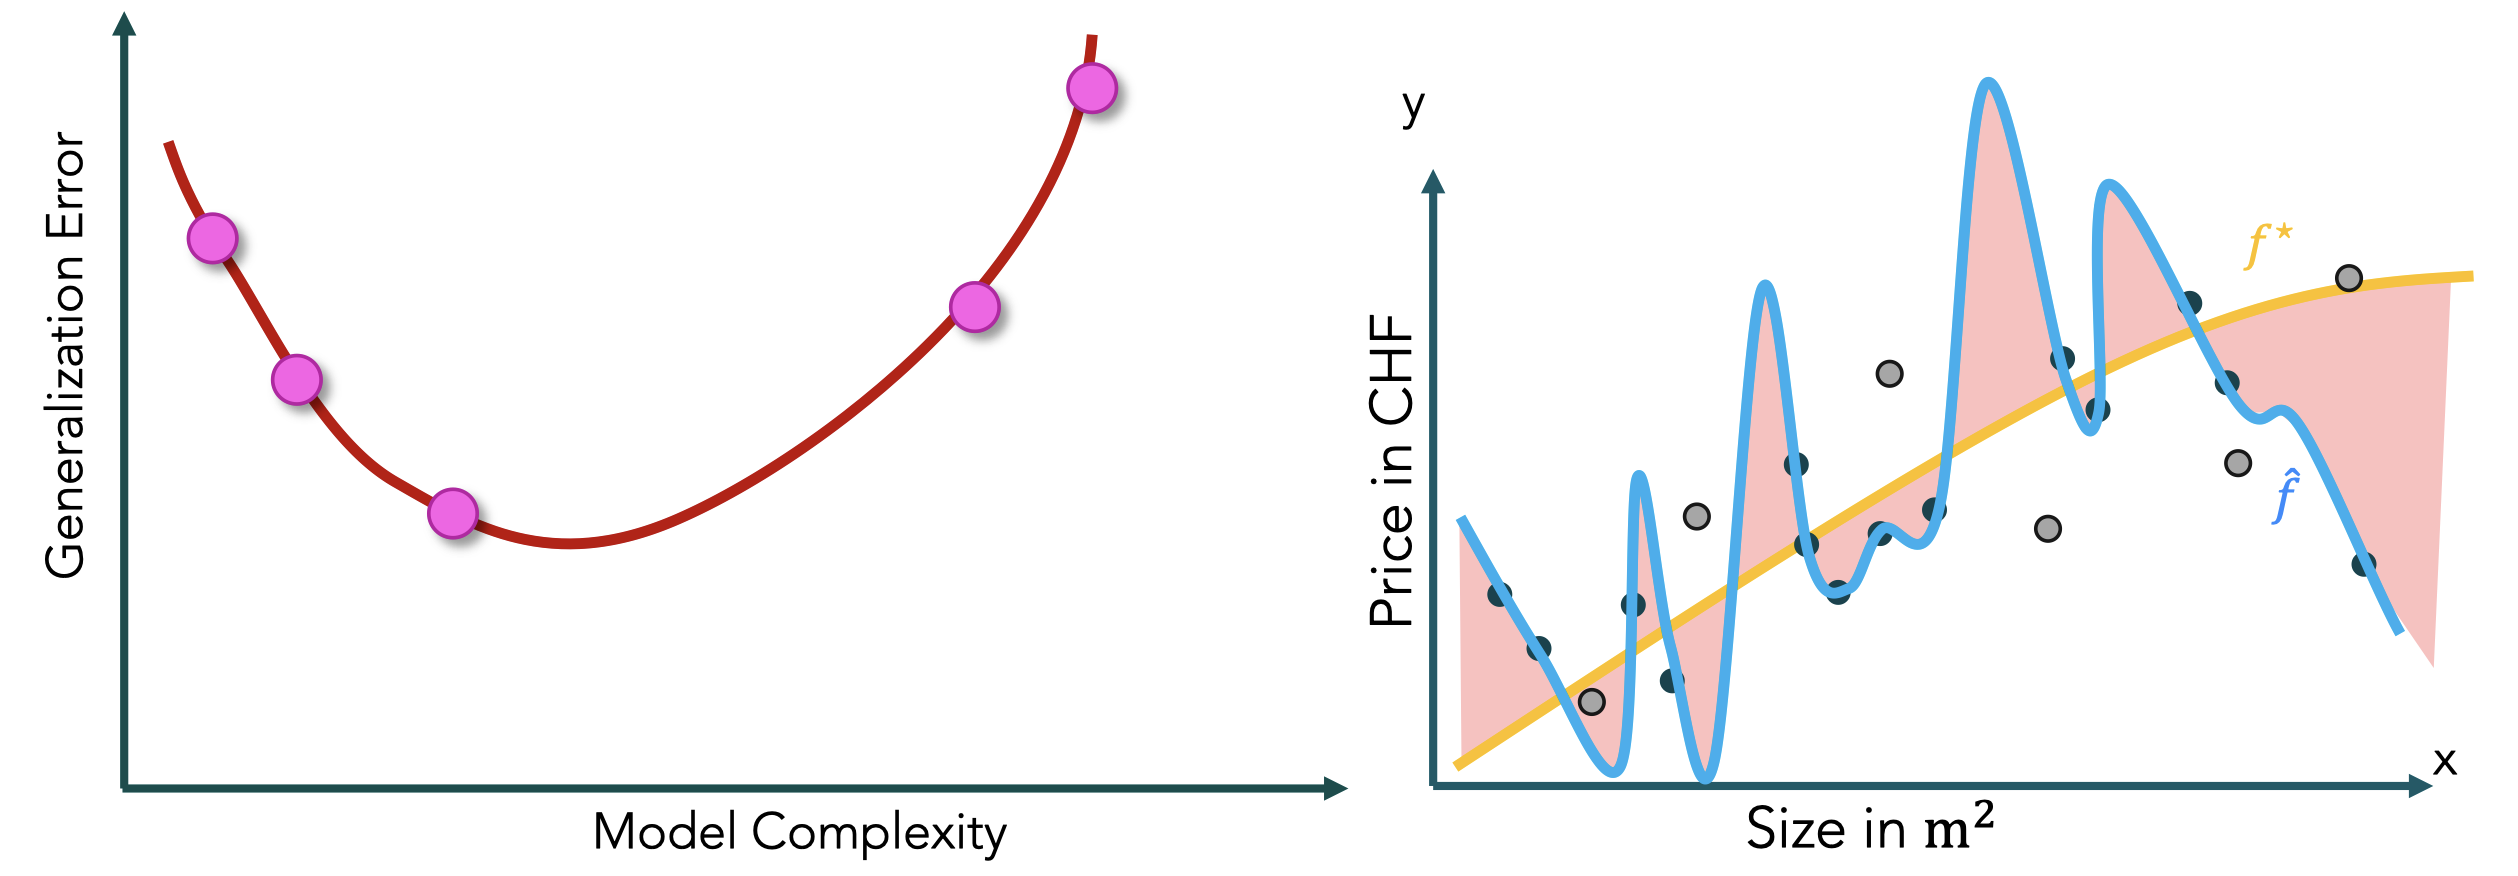
\includegraphics[width=15cm]{../images/IntroML_Fig3-15}
    \centering
\end{figure}

\subsubsection{Phenomenon of Under- and Overfitting}

\begin{figure}[H]
    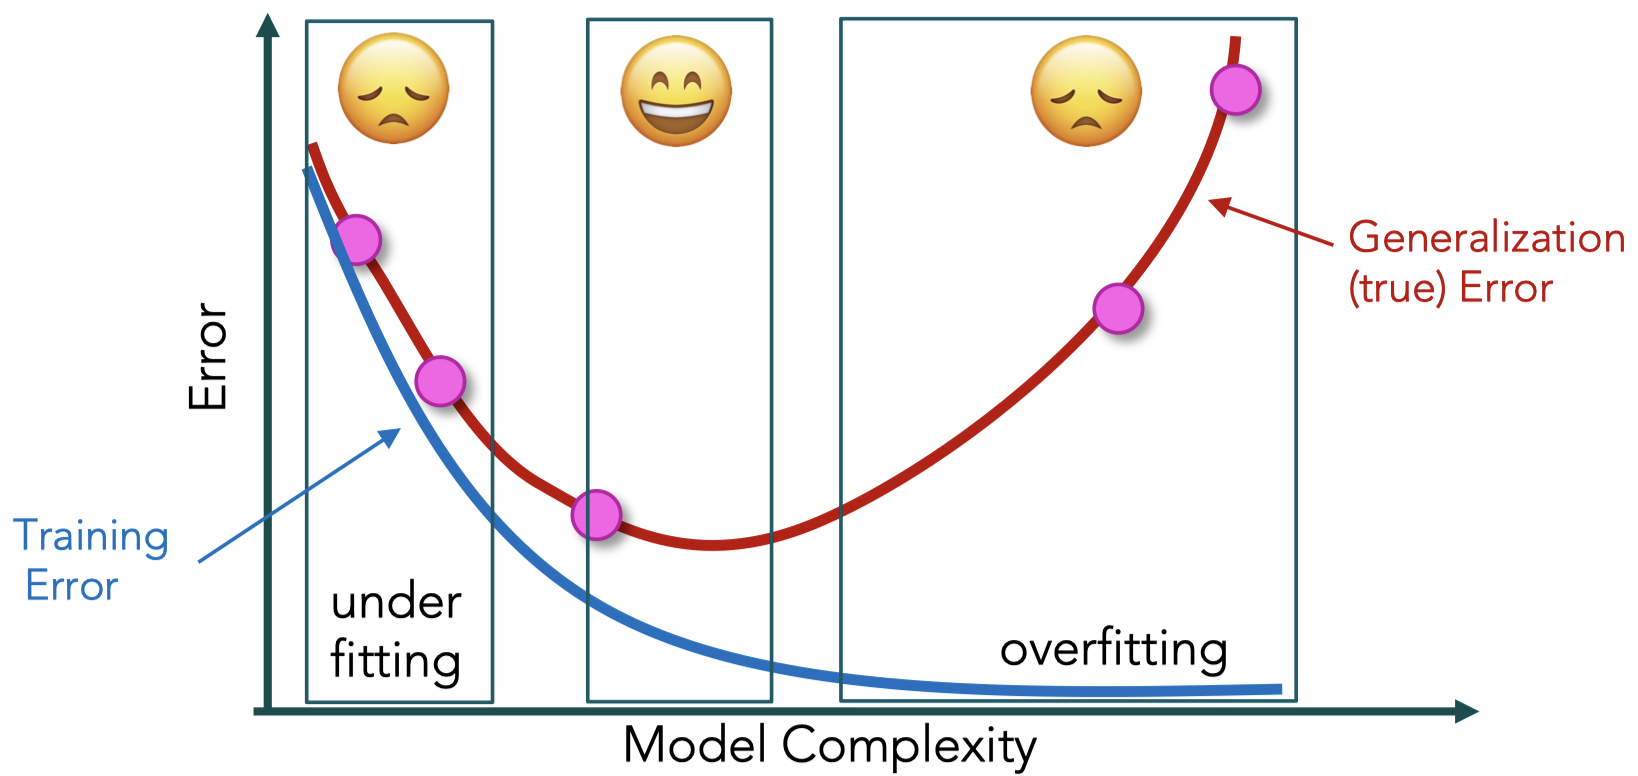
\includegraphics[width=11cm]{../images/IntroML_Fig3-16}
    \centering
\end{figure}

In summary:

\begin{itemize}
    \item Underfitting models predict: training data not well, and test data not well
    \item The "right" model predicts: training data well, and test data well
    \item Overfitting models predict: training data very well, test data not well
\end{itemize}

\section{Bias-Variance Tradeoff \& Regularization}

\subsection{Bias-Variance Decomposition}

\subsubsection{Bias}

The \textbf{bias} of some method \(M\) is the distance of the average model \(\bar{f} = \frac{1}{K} \sum_{k = 1}^K \hat{f}_k\) to the ground truth \(\mathbb{E}_x (f^*(x) - \bar{f}(x))^2\).

\begin{figure}[H]
    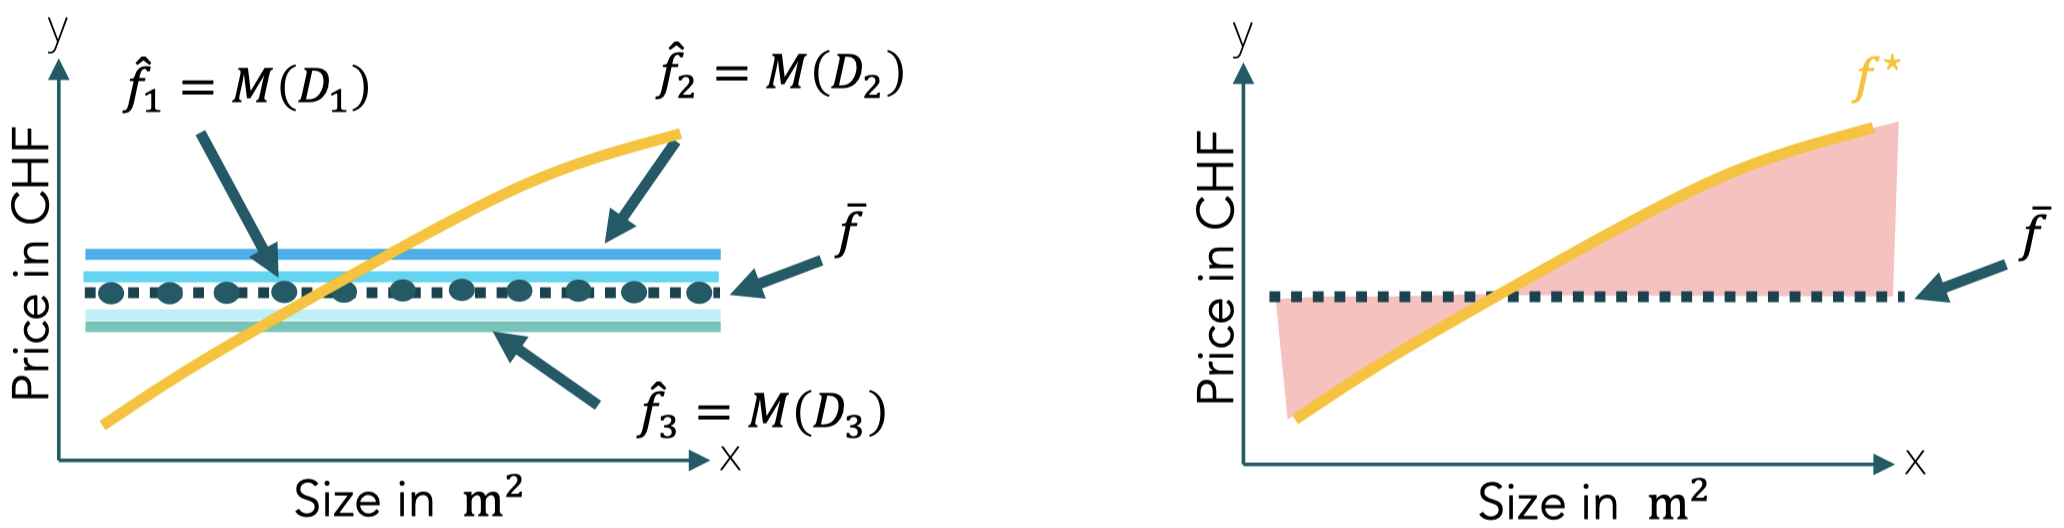
\includegraphics[width=15cm]{../images/IntroML_Fig3-17}
    \centering
\end{figure}

It is important to note that complex functions can model the ground truth well on average, as shown by the following figure:

\begin{figure}[H]
    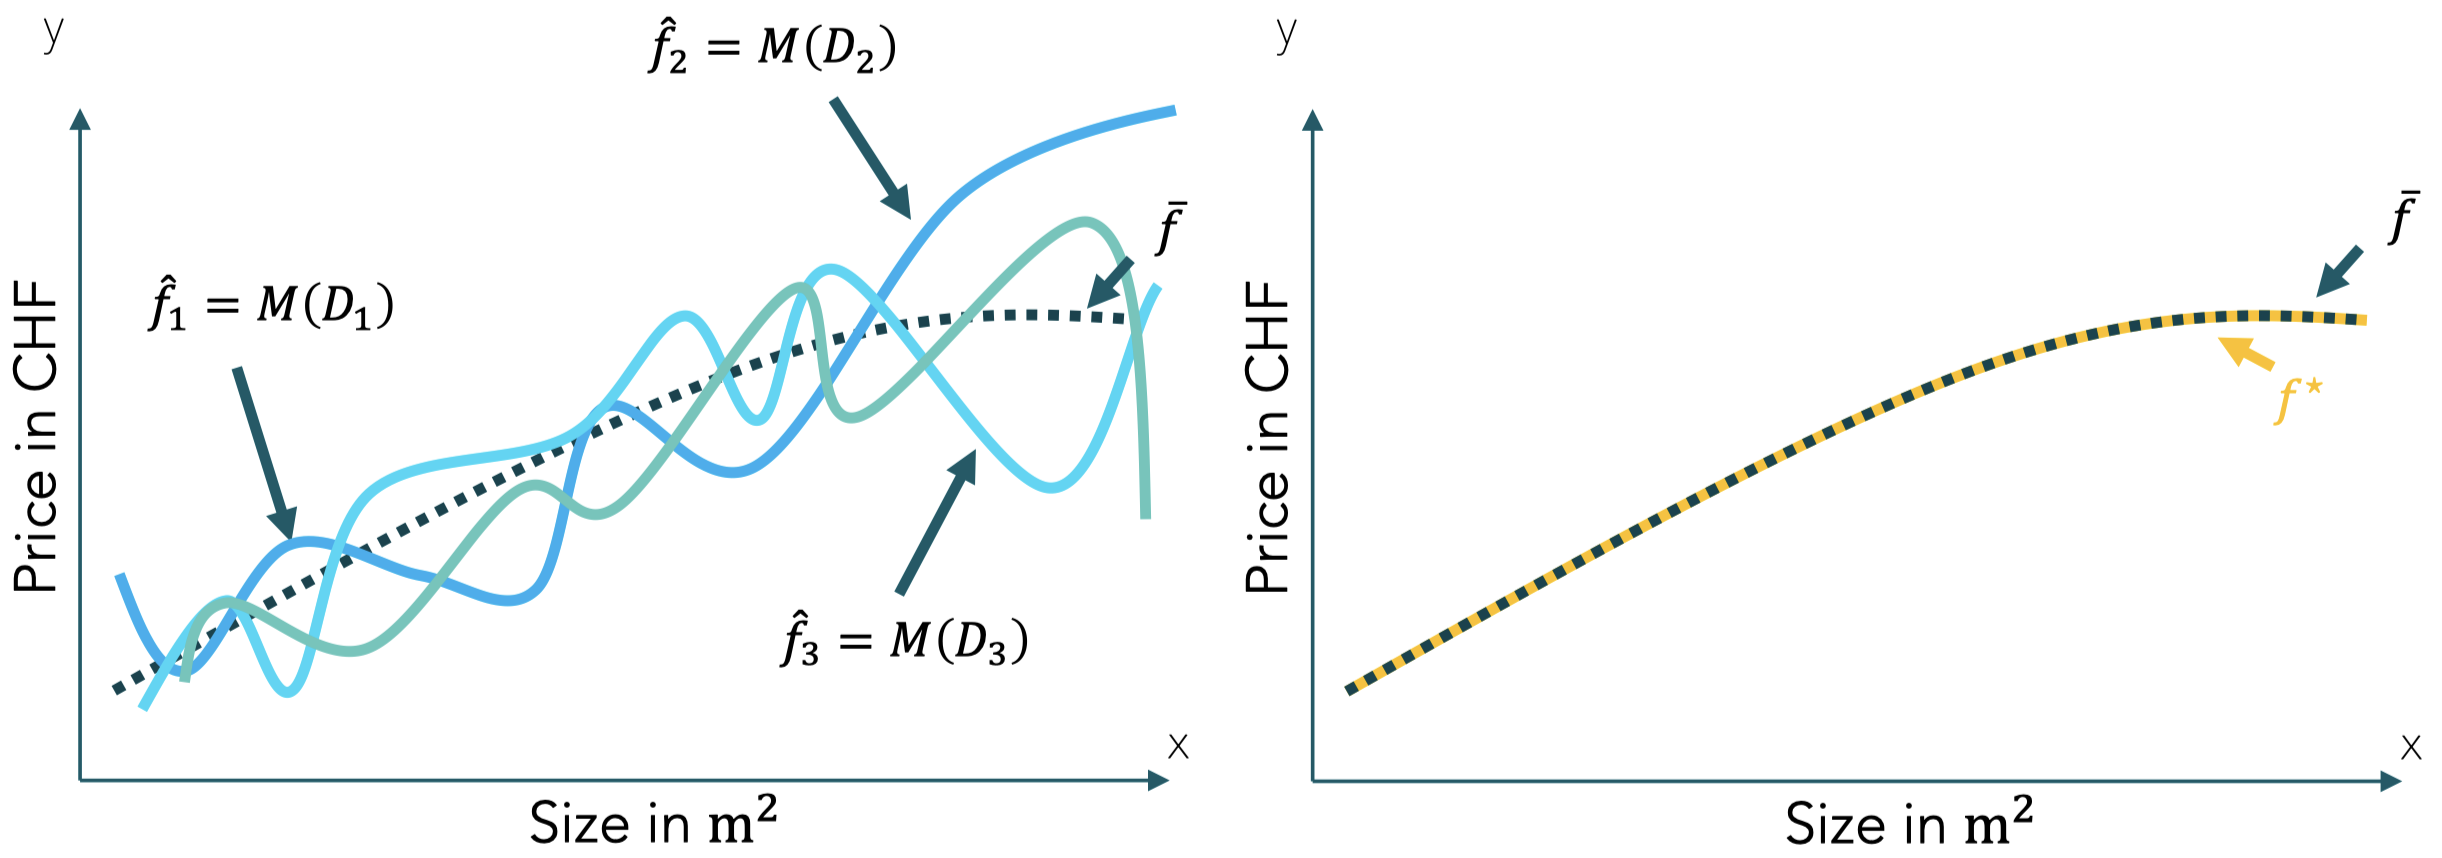
\includegraphics[width=15cm]{../images/IntroML_Fig3-18}
    \centering
\end{figure}

\subsubsection{Variance}

The \textbf{variance} of some method \(M\) is the average distance of individual models to the average model, i.e. \(\mathbb{E}_x \frac{1}{K}\sum_{k = 1}^K (\hat{f}_k(x) - \bar{f}(x))^2\). For complex models, the varaince is large, whereas it is small for simple models:

\begin{figure}[H]
    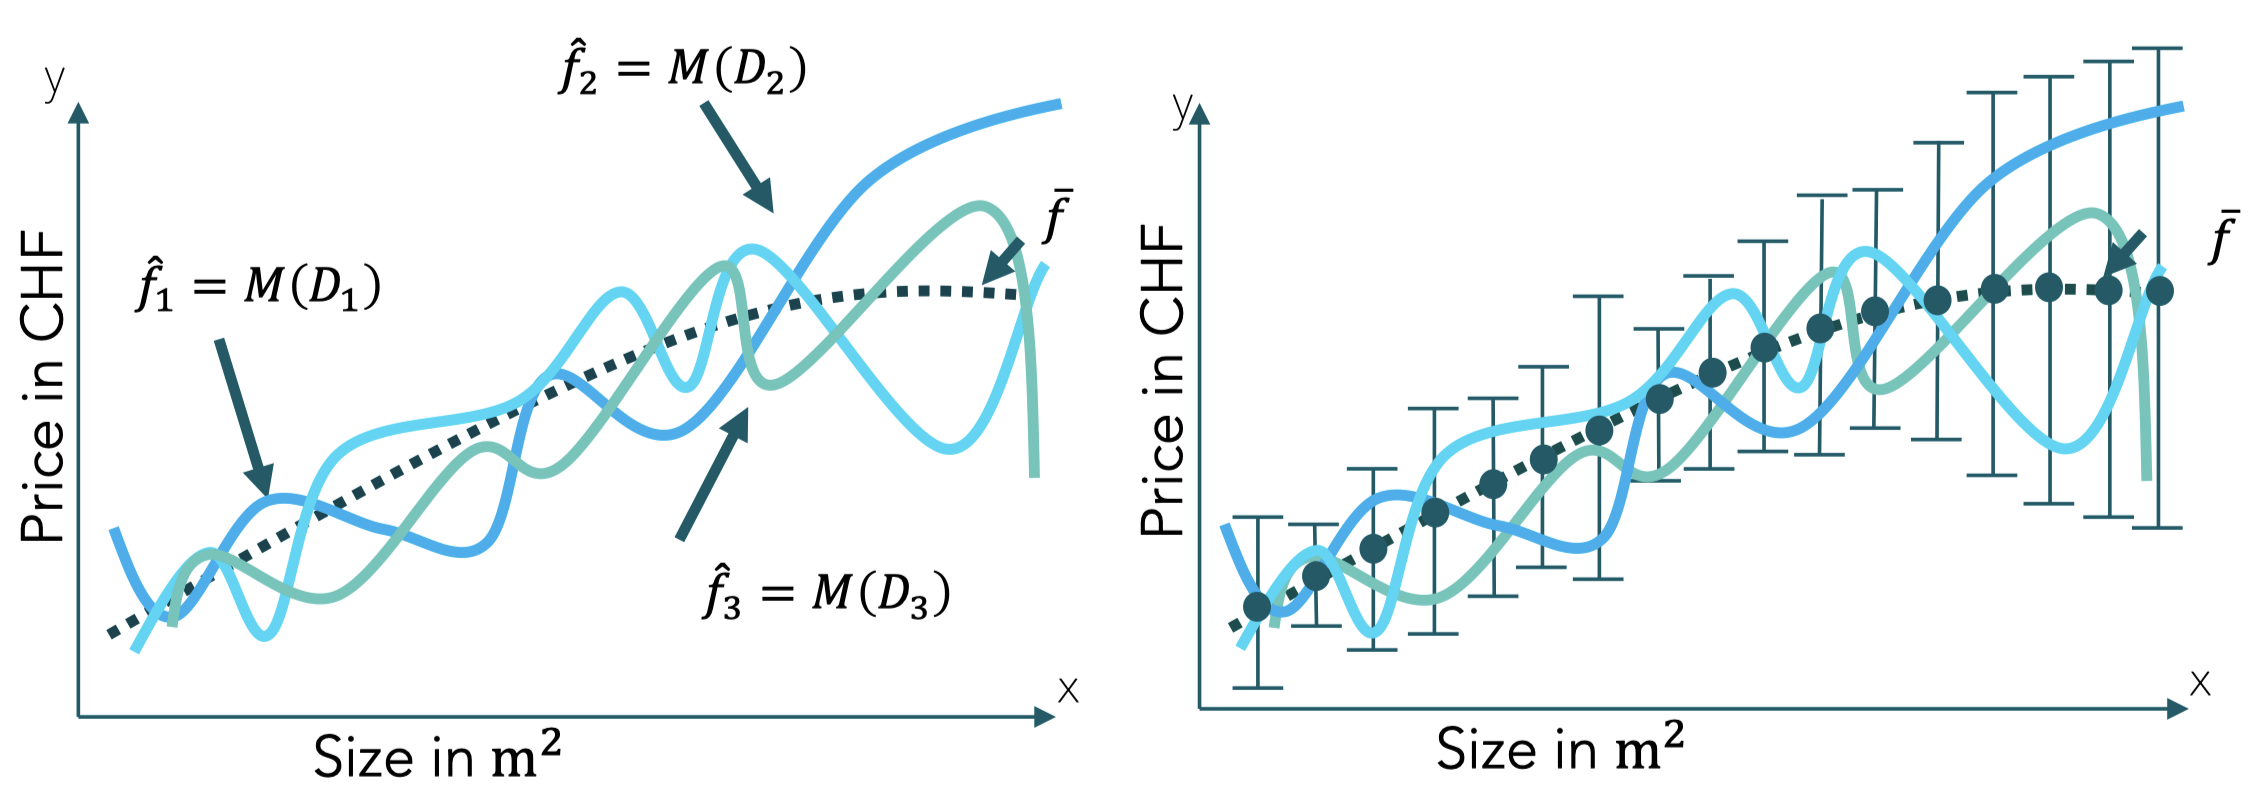
\includegraphics[width=15cm]{../images/IntroML_Fig3-19}
    \centering
\end{figure}

\begin{figure}[H]
    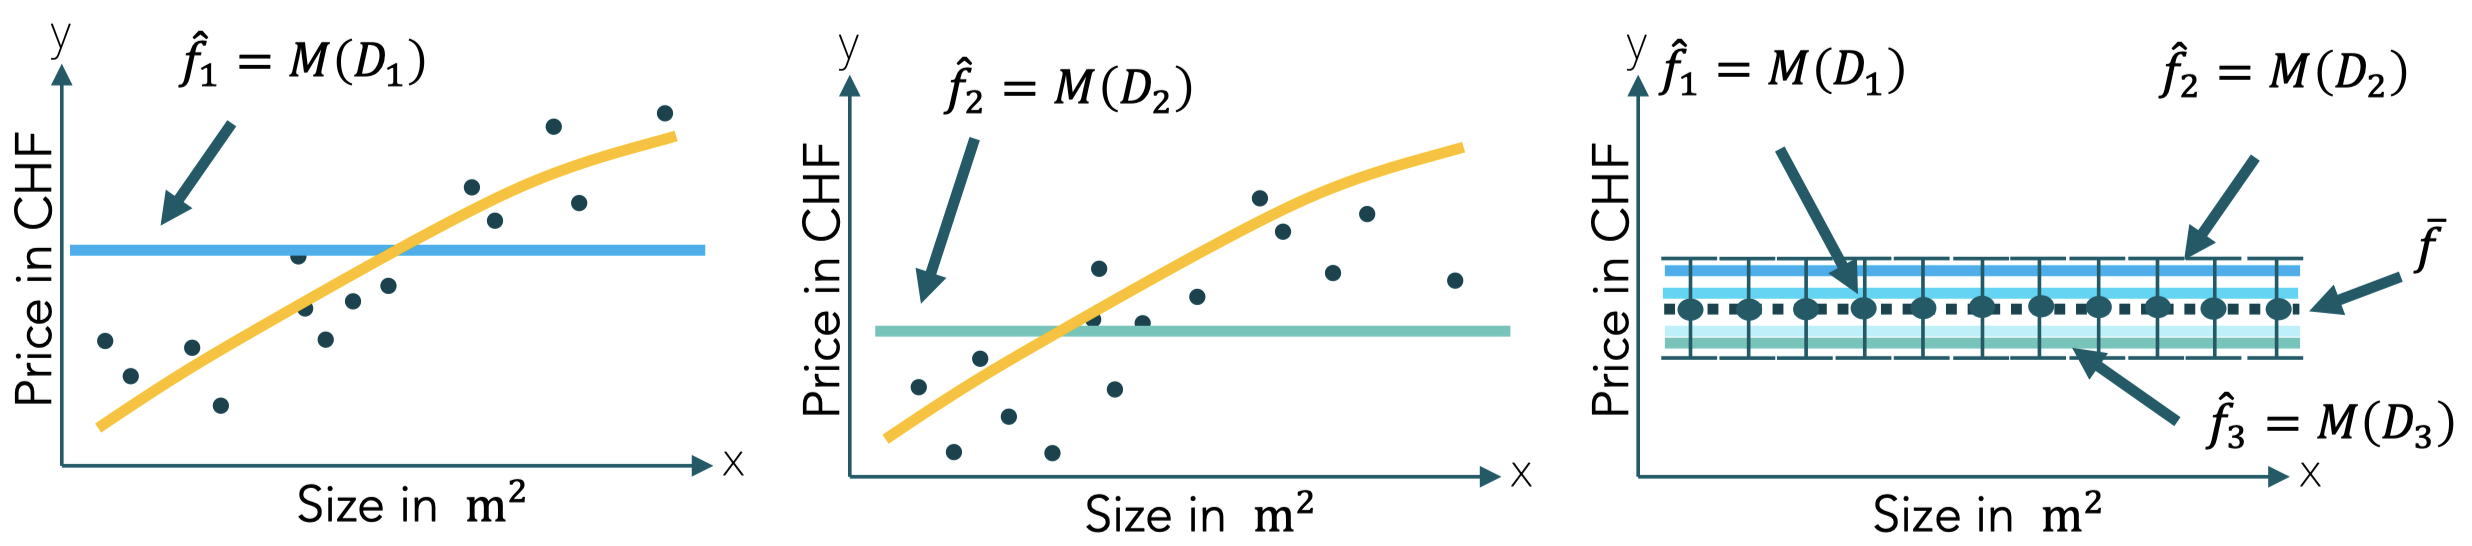
\includegraphics[width=15cm]{../images/IntroML_Fig3-20}
    \centering
\end{figure}

\subsubsection{Conclusion}

In summary:

\begin{itemize}
    \item Bias = "average - ground truth"
    \begin{itemize}
        \item Drives Underfitting
        \item Arises even for noiseless data
    \end{itemize}
    \item Variance = "individual - average"
    \begin{itemize}
        \item Drives overfitting
        \item Especially for complex models
    \end{itemize}
\end{itemize}

\subsection{Regularization}

\subsubsection{Different Methods}

Given a setting with linear regression with \(1d\) polynomial features \(\phi(x) = (1, \, x, \, x^2,..., \, x^m)\). We observe that complex models use too many features! But how can we force it to use fewer?

Ideally we have that \(\arg \min_{w \in \mathbb{R}^d} ||y - \Phi w||^2\) is such that \(||w||_0 \leq k\). I.e. we need to search for the best subset of size \(k\), however this is combinatorial infeasible for large \(d\).

The option we choose is to only use a few of these features and encourage sparsity via limiting the \(l_1\)-norm through \textbf{lasso regression:}

\[
    \arg \min_{w \in \mathbb{R}^d} ||y - \Phi w||^2 \quad s.t. \, ||w||_1 \leq R \Leftrightarrow \arg \min_{w \in \mathbb{R}^d} ||y - \Phi w||^2 + \lambda ||w||_1
\]

Another option would be to choose models with limited \(l_2\)-norm through \textbf{ridge regression:}

\[
    \arg \min_{w \in \mathbb{R}^d} ||y - \Phi w||^2 \quad s.t. \, ||w||_2 \leq R \Leftrightarrow \hat{w}_{\lambda} = \arg \min_{w \in \mathbb{R}^d} ||y - \Phi w||^2 + \lambda ||w||_2^2,
\]

where \(R\) is given and equivalent for some \(\lambda\). The \textit{closed-form solution} is simple by finding the stationary point: \(\hat{w}_{\lambda} = (X^TX + \lambda I)^{-1}X^Ty\)

\subsubsection{Intuition Behind the Lasso}

The first inuition can be given with small calculations. Take for example \(w_{sparse} = (1, \, 0, \, 0,..., \, 0)\) vs. some dense vector \(w_{dense} = \frac{1}{\sqrt{d}}(1, \, 1, \,..., \, 1)\). For the same \(l_2\) norm, the vectors with the smallest \(l_1\) norm are sparse

\[
    ||w_{dense}||_1 = \sqrt{d} >> ||w_{sparse}||_1 = 1,
\]

whereas vectors with the largest \(l_1\) norm are dense

\[
    ||w_{dense}||_1 = \sqrt{d} >> ||w_{dense}||_2 = 1.
\]

\begin{figure}[H]
    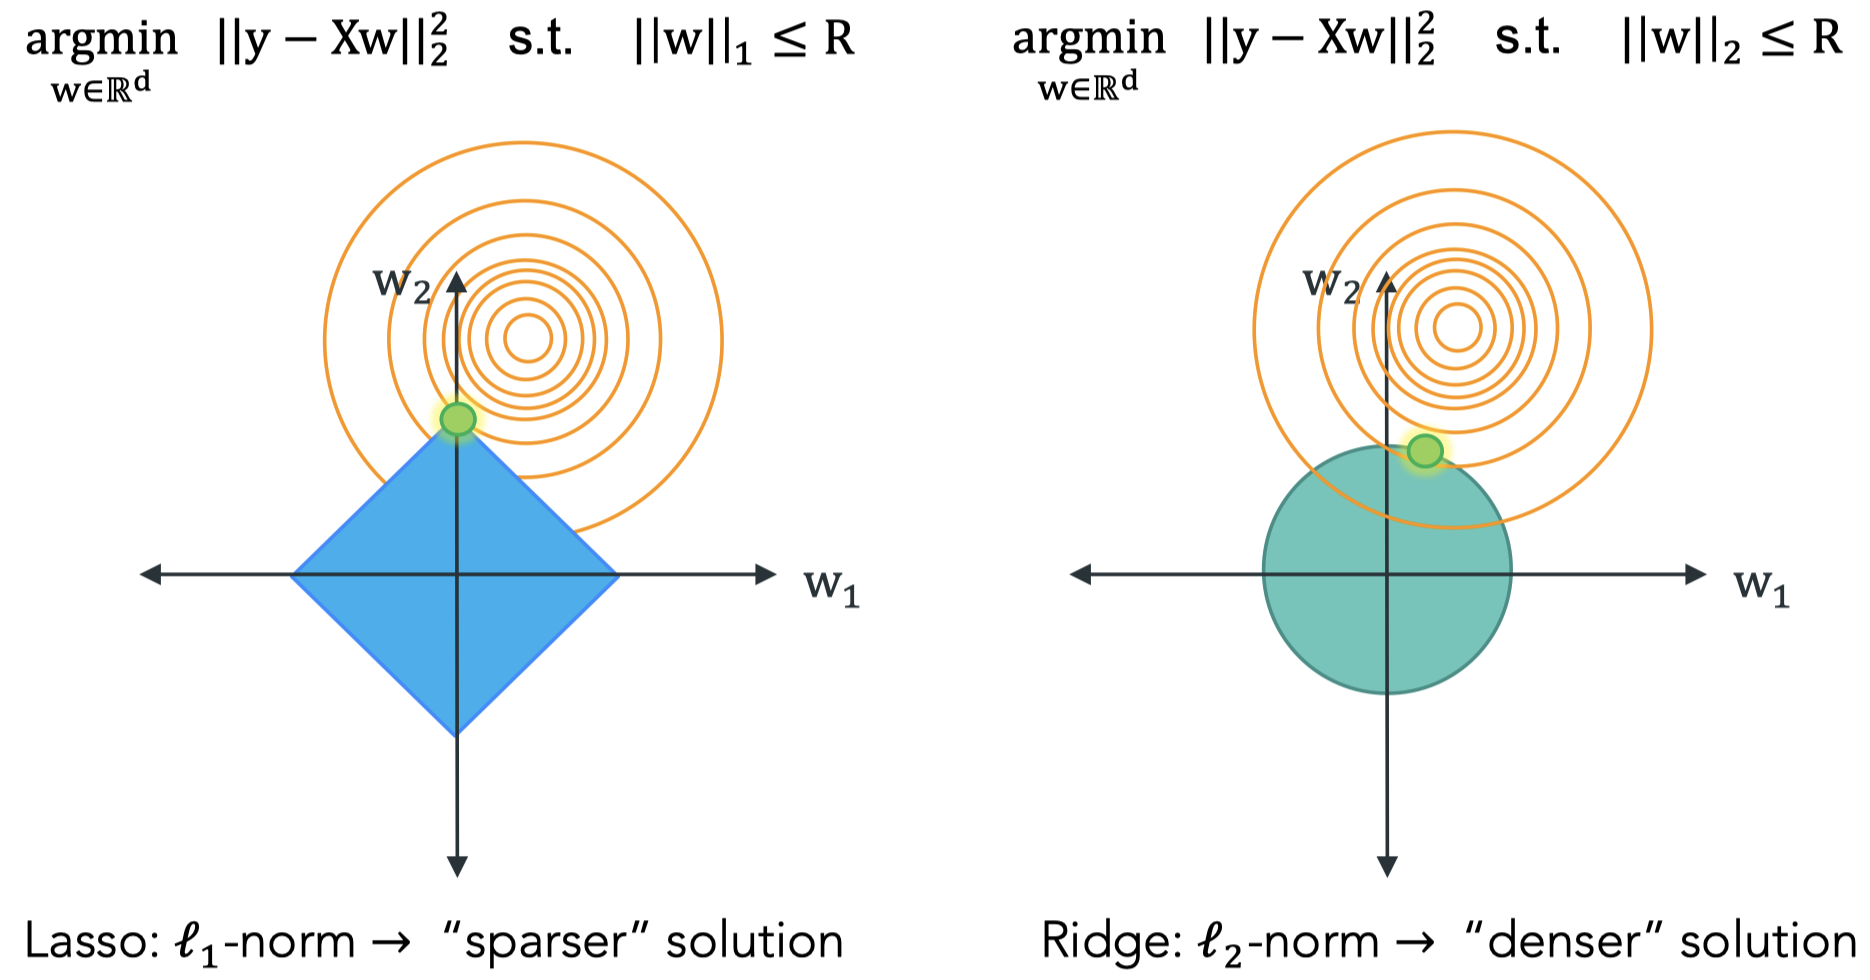
\includegraphics[width=15cm]{../images/IntroML_Fig3-21}
    \centering
\end{figure}

\subsubsection{Bias and Variance as Function of Regularization Strength}

The variance shrinks and the bias increases with model complexity. The following figure shows varying model complexity reflected via sizes of ellipses for \(n > d\):

\begin{figure}[H]
    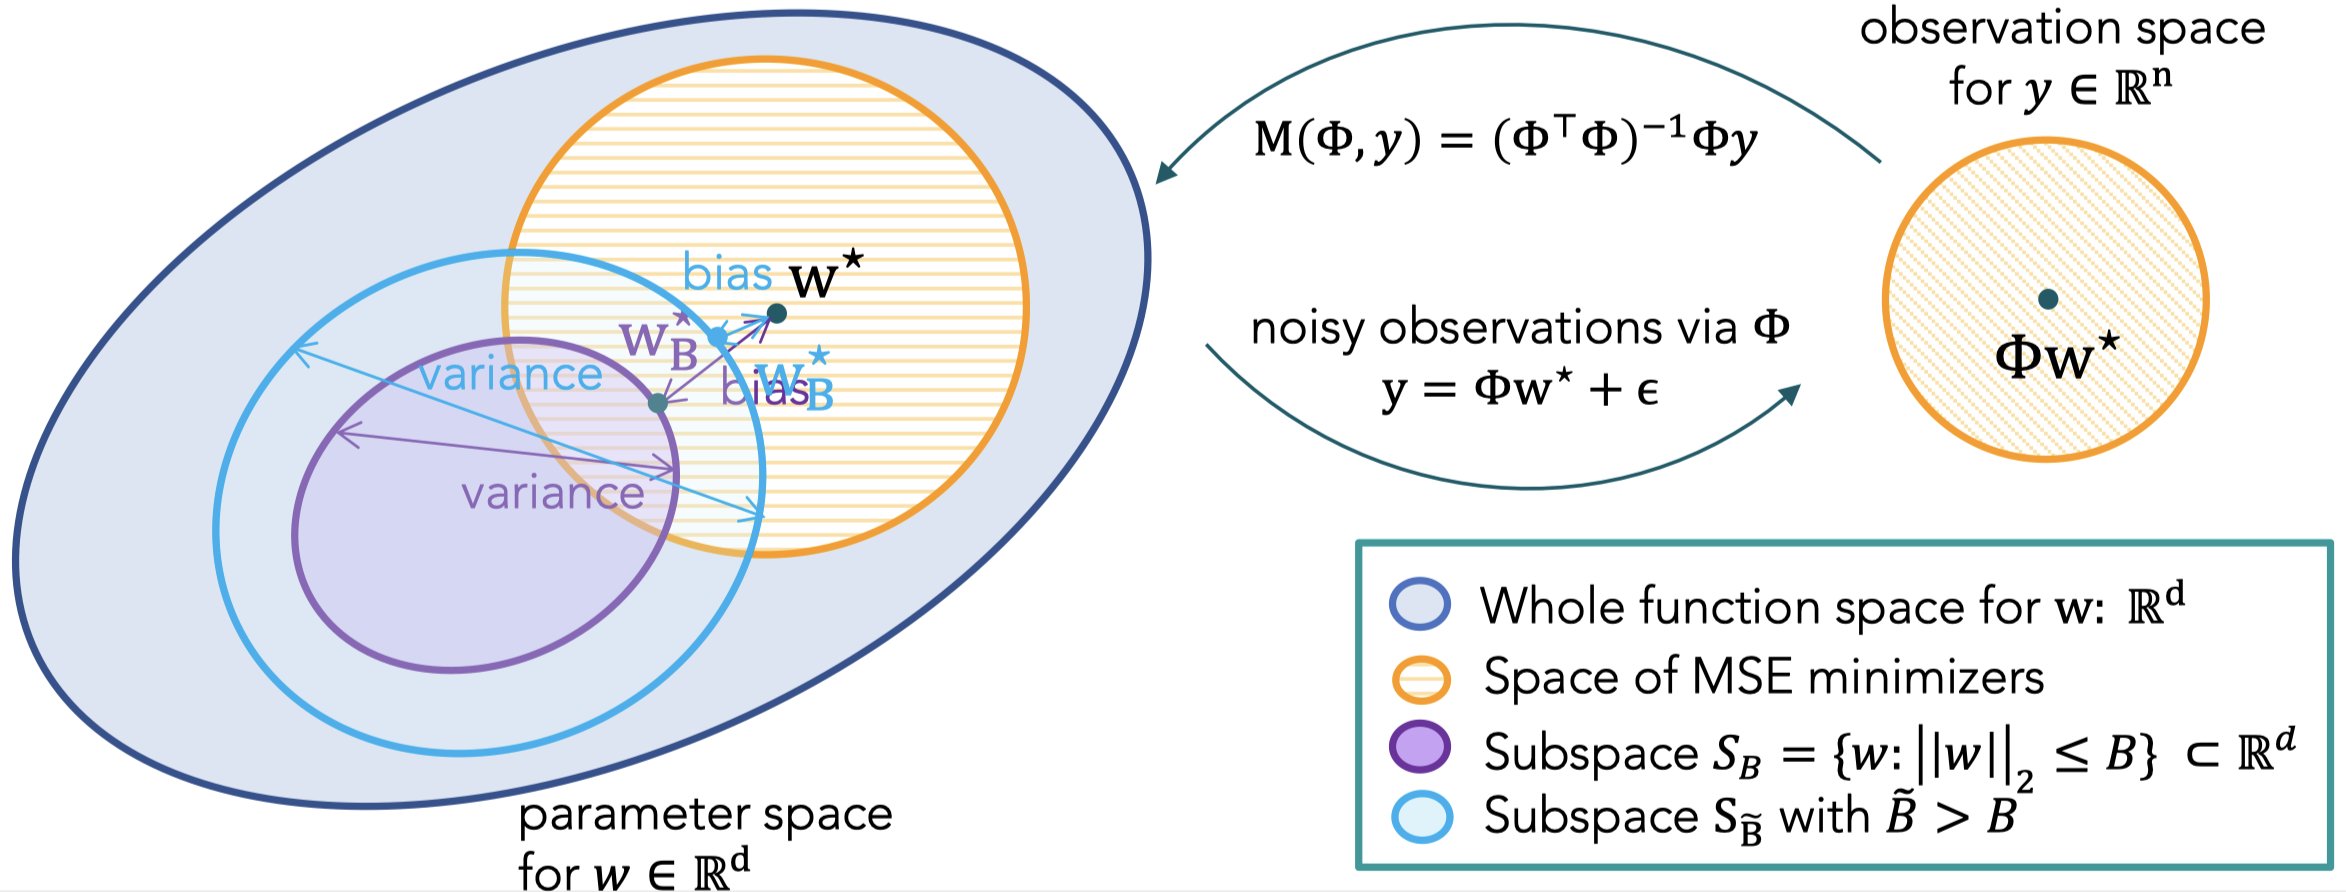
\includegraphics[width=15cm]{../images/IntroML_Fig3-22}
    \centering
\end{figure}

We might also display the bias and variance as a function of \(\lambda\):

\begin{figure}[H]
    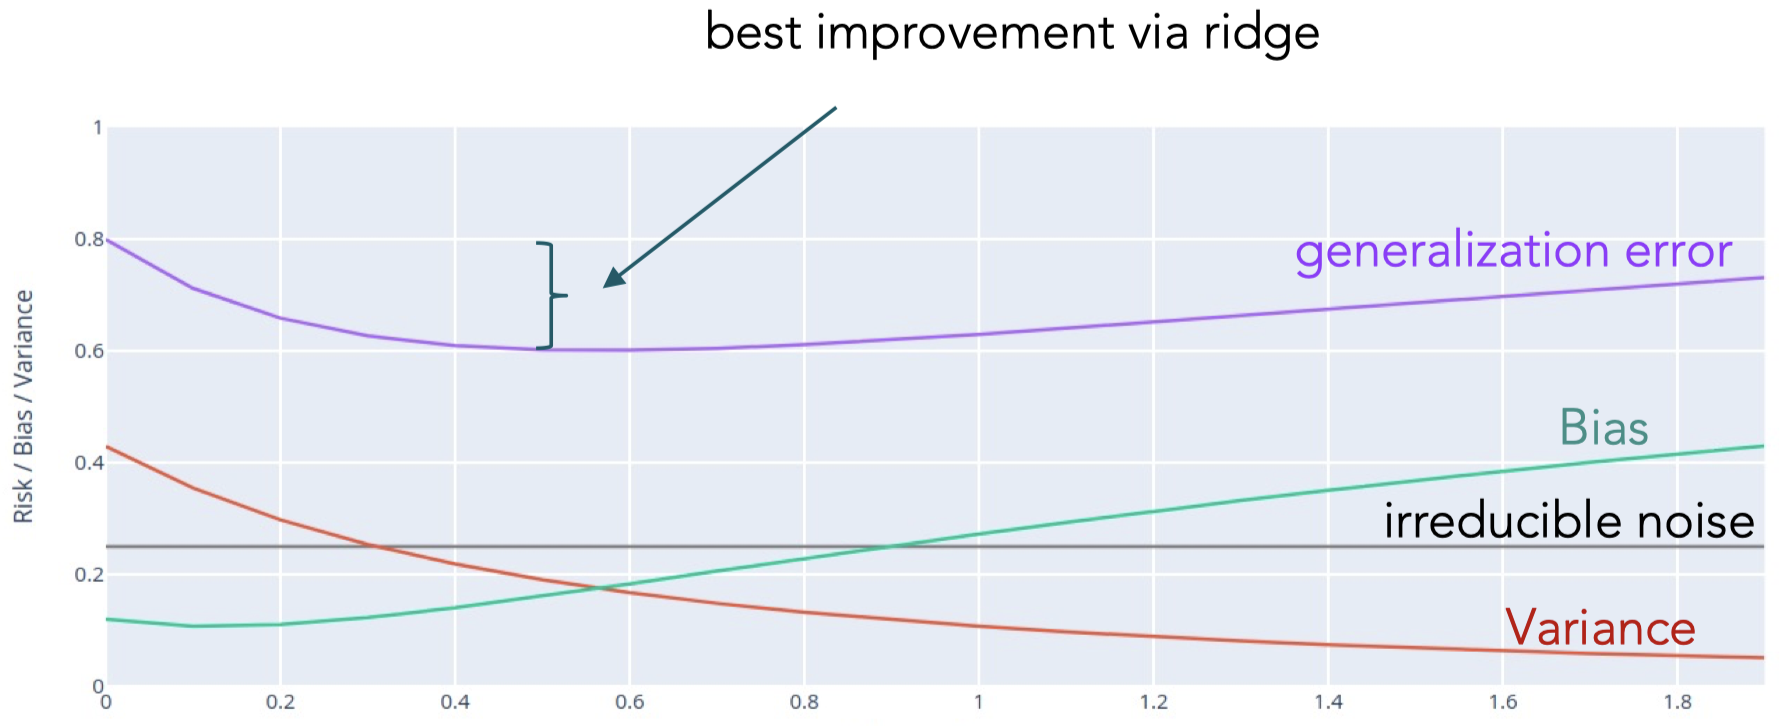
\includegraphics[width=15cm]{../images/IntroML_Fig3-23}
    \centering
\end{figure}

\subsubsection{Cross-Validation to Determine Regulariztaion Strength}

Instead of feature maps. the question now becomes how to optimally choose \(\lambda\).

The regularized estimator \(\hat{f}^{\lambda} = \langle \hat{w}_{\lambda}; \cdot \rangle = M_{\lambda}(D)\) is the minimizer of the regularized training loss \(M_{\lambda}(D) = \arg \min_f L_0 (f; \, D) + \lambda ||f||\) with \(L_0 (f, \, D) = \frac{1}{|D|} \sum_{(x, \, y) \in D} l(f(x), \, y)\).

The algorithm is the same as before:

\begin{cbox}
    \textbf{Algorithm:} Given a choice of features \(\lambda\), and \(K\) folds, do the following steps:
    \begin{enumerate}
        \item For all folds \(k = 1,..., \, K\)
        \begin{enumerate}
            \item Compute \(\hat{f}^{\lambda}_k = M_{\lambda}(D_k) = \arg \min_f L_0(f; \, D_k) + \lambda ||f||\)
            \item Compute validation loss on fold \(k : R_{k}(\lambda) = \frac{1}{|D'_k|}\sum_{(x, \, y) \in D'_k}l(\hat{f}^{\lambda}_k)(x), \, y\)
        \end{enumerate}
        \item Compute cross-validation error \(CV_K(\lambda) = \frac{1}{K} \sum_{i = 1}^K R_k(\lambda)\)
        \item Model selection: Pick \(\lambda\) with lowest error \(CV_k(\lambda)\)
        \item Model training: Compute final model \(\hat{f} = \hat{f}^{\lambda} = M_{\lambda}(D_{rest})\)
        \item Model evaluation: Estimate generalized error using \(D_{test}\)
    \end{enumerate}
\end{cbox}

\end{document}